\cotefile{6}
\scanpage{38}

Gribouillis de Tate
sur sa théorie

\margin{37}

\scanpage{40}

Questions diverses en
théorie de Tate-Hodge

\margin{50}

\scanpage{41}

\uline{\unsure{Questions|Question}} a) Trouver un \unsure{isom.}
(\unsure{fonctoriel}-multiplicatif en $X$, \unsure{?} commutant aux \unsure{homom\textsuperscript{t}} de structure)
\[
H_{DR}(X_C) \simeq H_{Hdg}(X_C)
\]
compatible aux filtrations --- du moins une fois \unsure{donné|choisi} un \inserted{générateur} $\varepsilon\in T_\ell(C^*)$ ? \deleted{\illegible{1}}

b) Tout $Q_\ell(\pi)$-module simple, de dim finie sur $Q_\ell$, est-il contenu dans un $C(i)$ ?
$C\deleted{\unsure{(i)}}$ peut-il contenir à la fois un $M$ et un $M(i)$, pour $i\ne0$ ??

c) Y-a-t-il d'autres conditions sur les
\[
M=H^i(X_C,\mathbb Z_\ell)\otimes_{\mathbb Z_\ell}Q_\ell
\]
que celles résultant de la conjecture de Tate ?

d) \uline{\unsure{Construire|Conditions}} les isomorphismes de Tate
\[
H_B^{\unsure{pq|p+q}}(X)_{\unsure{\chi}}\simeq H^q(X,\Omega_X^p)
\]

e) Lien de \unsure{ttes} ces structures avec les connexions canoniques ??

f) Lien avec Washnitzer-Monsky ?

\margin{51}

\scanpage{42}
\mspage{- 15 -}
\margin{n°357}

déterminée par cette même norme ; son dual est alors $\mathcal M_b^1(E)$, espace des mesures bornées sur $E$.

PROPOSITION 5.- \uline{Soit} $G$ \uline{un groupe localement compact opérant sur un espace} $E$ \uline{localement compact} ; \uline{pour tout} $x\in G$, \uline{soit} $\varphi_x$ \uline{l'automorphisme} $z\to xz$ \uline{déterminé par} $x$ \uline{dans} $E$. \uline{Alors les applications} $(x,f)\to f\circ\varphi_x$ \uline{de} $G\times\mathcal K(E)$ \uline{dans} $\mathcal K(E)$, \uline{et de} $G\times\overline{\mathcal K(E)}$ \uline{dans} $\overline{\mathcal K(E)}$, \uline{sont continues}.

Soit $V$ un voisinage de $0$ dans $\mathcal K(E)$ ; il y aura donc, pour tout compact $K$ dans $E$, un $\delta(K)>0$ tel que $f\in V$ chaque fois que $\sup_E|f|\le\delta(K)$ et que le support de $f$ est contenu dans $K$. Soient $x_0$ un point de $G$ et $K_0$ un voisinage compact de $x_0$ dans $G$. Soit $W$ l'ensemble des $g\in\mathcal K(E)$ tels que la fonction $z\to 2g(xz)$ appartienne à $V$ quel que soit $x\in K_0$ ; c'est un voisinage de $0$ dans $\mathcal K(E)$, car $W$ est convexe et symétrique, et, si $K$ est compact, tout $g$ de support contenu dans $K$ et tel que $\sup_E|g|\le\delta(K_0^{-1}K)/2$ est dans $W$. Soit $f_0\in\mathcal K(E)$ ; soit $K'$ son support ; soit $K''=K_0^{-1}K'$ ; pour tout $x\in K_0$, le support de $z\to f_0(xz)$ est contenu dans $K''$ ; la fonction $(x,z)\to f_0(xz)$ étant uniformément continue sur $K_0\times K''$, il y a un voisinage $U$ de $x_0$ dans $K_0$ tel que l'on ait
\[
|f_0(xz)-f_0(x_0z)|\le\delta(K'')/2
\]
pour tout $x\in U$ et tout $z\in K''$ ; donc, pour $x\in U$, la fonction
\[
z\to 2f_0(xz)-2f_0(x_0z)
\]
appartient à $V$. Comme $V$ est convexe, on en conclut que, si l'on pose $f=f_0+g$, la fonction $f\circ\varphi_x-f_0\circ\varphi_{x_0}$ est dans $V$ quels que soient $x\in U$ et $g\in W$, ce qui démontre la première partie de la proposition. La démonstration de la seconde est analogue mais plus simple, et est laissée au lecteur pour son amusement.

COROLLAIRE.- \uline{Soit} $G$ \uline{un groupe localement compact opérant sur un espace loca-}

\margin{52}

\scanpage{43}

\margin{\figure{\begin{tikzpicture}[x=1cm,y=1cm]\draw (0.7,1.7)--(0,0)--(0.7,-1.7);\end{tikzpicture}}}

1) $V=V^{10}+V^{01}$ \unsure{décomposition de vectoriels} sur $C$

\deleted{1') $V^{10}\simeq\unsure{\check V^0}\otimes C,\quad V^{01}\simeq\unsure{\check V^1}\otimes_K C[-1]$}

2) Opération de $\pi$ sur $V$, \unsure{comp. aux op. de $\pi$ sur $C$}.

3) $V\simeq M\otimes_{\mathbb Z_p}C$, $M$ un \deleted{\unsure{vectoriel|réseau}} \inserted{module libre de t.f.} sur $\mathbb Z_p$.

\uline{Relations}

\uline{1) et 2)}
\[
V^{10}=V^\pi\otimes_K C
\]
\[
V^{01}=(V\otimes C[1])^\pi\otimes_K C[-1]
\]
\margin{\uline{NB} Structures $1,2$ \unsure{reviennent à un couple} $\unsure{\check V^0}=V^\pi$, $\unsure{\check V^1}=(V\otimes C(1))^\pi$.
NB. $2\unsure{\not\Rightarrow|\Rightarrow}1$}

\uline{2) et 3)} $M$ stable par $\pi$
\margin{[NB. \unsure{Structures $2,3$. connues} \inserted{\unsure{donne aussi 1)}} quand on \unsure{donne} $M$ avec op. de $\pi$ dessus
\deleted{\unsure{NB.} \illegible{2}} (i.e. le grp $p$-divisible \unsure{sur} $K$)]}

\uline{3 et 1} ??? \deleted{Les autom. de $M$ \unsure{qui sont compatibles}}

\uline{NB} le corps $K$ intervient dans 2), du moins \unsure{implicitement}, mais pas dans 1), ni 3), qui \unsure{semblent} des structures intrinsèques : la donnée du groupe $p$-divisible sur
\[
\unsure{\widehat S}\subset\widehat\Omega=C.
\]

Regardons le \inserted{plus petit} groupe \unsure{alg.} d'autom. \inserted{$G$} de $M\otimes Q_\ell$ \deleted{\unsure{qui}} tel que $G_C$ contienne les opérations
$\begin{pmatrix}\lambda&0\\0&\unsure{1|\xi}\end{pmatrix}$ pour la décomposition de $V$ en $V^{10}+V^{01}$.

\margin{53}

\scanpage{44}
\mspage{- 27 -}
\margin{n° 380}

PROPOSITION 3.- \uline{Pour toute fonction} $f$ \uline{holomorphe sur un voisinage du spectre de} $x\in A$, \uline{on a} $\operatorname{Sp}(f(x))=f(\operatorname{Sp}(x))$.

Supposons en effet que $t\in\operatorname{Sp}(x)$. Alors $f(z)-f(t)$ est holomorphe sur un voisinage de $\operatorname{Sp}(x)$ et est nulle au point $z=t$. Il existe donc une fonction $g(z)$ holomorphe sur un voisinage de $\operatorname{Sp}(x)$ telle que $f(z)-f(t)=g(z)(z-t)$. On en déduit que $g(x)(x-te)=f(x)-f(t)e$. (Propositions 1 et 2). Puisque $(x-te)$ n'est pas inversible dans $A$, il en résulte que $f(x)-f(t)e$ n'est pas inversible dans $A$ donc que $f(t)\in\operatorname{Sp}(f(x))$. Réciproquement, si $t\notin f(\operatorname{Sp}(x))$, alors $h(z)=(f(z)-t)^{-1}$ est holomorphe sur un voisinage de $\operatorname{Sp}(x)$. On a donc $h(x)(f(x)-te)=e$, ce qui prouve que $t\notin\operatorname{Sp}_{(f(x))}$.

COROLLAIRE.- \uline{Pour que} $f(x)$ \uline{soit inversible dans} $A$, \uline{il faut et il suffit que} $0\notin f(\operatorname{Sp}(x))$.

PROPOSITION 4.- \uline{Soient} $x$ \uline{un élément de} $A$, $f$ \uline{une fonction holomorphe sur un voisinage} $U$ \uline{de} $\operatorname{Sp}(x)$ \uline{et} $g$ \uline{une fonction holomorphe sur un voisinage} $V$ \uline{de} $f(\operatorname{Sp}(x))$. \uline{Alors} $(g\circ f)(x)=g(f(x))$.

Soient $d\mu$ une mesure à support compact contenu dans $V\cap(\mathbb C-f(\operatorname{Sp}(x))$ et $W$ un voisinage ouvert de $f(\operatorname{Sp}(x))$ tels que pour tout $z\in W$, on ait $g(z)=\frac{d\mu(\theta)}{z-\theta}$. Soient d'autre part $d\rho$ une mesure à support compact contenu dans $U\cap f^{-1}(W)\cap(\mathbb C-\operatorname{Sp}(x))$ et $W^\circ$ un voisinage ouvert de $\operatorname{Sp}(x)$ tels que, pour toute fonction $F$ holomorphe sur $U\cap f^{-1}(W)$ et tout $z\in W^\circ$, on ait
\[
F(z)=\int\frac{F(t)}{z-t}\,d\rho(t).
\]
La fonction $g\circ f$ étant holomorphe sur $U\cap f^{-1}(W)$, on a
\[
(g\circ f)(x)=\int R(x,t)g(f(t))\,d\rho(t).
\]
Mais, pour tout $t$ appartenant au support de $d\rho$, $f(t)\in W$ et par conséquent

\margin{54}

\scanpage{45}

\uline{Conjecture} 1) $H_B^i(X_C,C)$ est somme \inserted{directe} des sous-espaces engendrés par les \unsure{vecteurs} $\chi^{-p}$-propres, de façon intrinsèque ; posant, pour $p+q=i$
\[
H_B^{p,q}(X)_K=H_B^i(X_C,C)[p]^\pi
\]
on a une décomposition en \unsure{somme}
\[
\boxed{H_B^i(X_C,C)\simeq\coprod_{p+q=i}H_B^{p,q}(X)_K\otimes_K C[-p]}
\]

2) On a un isom canonique
\[
\boxed{\varphi_K^{pq}:H_B^{pq}(X)_K\simeq H^{p.q}(X)\overset{\mathrm{dfn}}{=}H^q(X,\Omega_X^p)}
\]

\figure{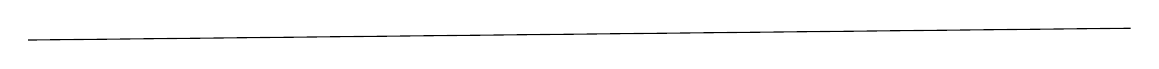
\begin{tikzpicture}\draw (0,0)--(14,0.15);\end{tikzpicture}}

\[
\begin{aligned}
\unsure{P_B|\rho_B}(z^i)&\in H_{\deleted{\unsure{B}}}^{2i}(X_C,\mathbb Z_p[i])^\pi
\subset H_B^{2i}(X_C,C)[i]^\pi=H_B^{i,i}(X)_K\\
&\phantom{\in H^{2i}(X_C,\mathbb Z_p[i])^\pi}\subset H_{\unsure{1}}^{2i}(X_C,\mathbb Z_p)
\end{aligned}
\]
\deleted{$\unsure{P_B|\rho_B}(z^i)$}
$\unsure{P_{DR}|\rho_{DR}}(z^i)\in H_{\deleted{\unsure{B}}}^{i,i}(X)$ ; on veut
\[
\boxed{\varphi_{\unsure{K}}^{ii}(\unsure{P_B|\rho_B}(z^i))=\unsure{P_{DR}|\rho_{DR}}(z^i)}
\]

\uline{NB.} On aura
\[
\unsure{P_B|\rho_B}(z^i)\in
\underbrace{H_B^{i,i}(\unsure{X_C,C})}_{\text{identifié à }H^{i,i}(X)}
\cap H^{2i}(X_C,\mathbb Z_p[i])
\]

\margin{55}

\scanpage{46}
\mspage{- 23 -}
\margin{n° 380}

§ 2. \uuline{Calcul fonctionnel holomorphe}.

1. \uline{Homomorphisme} $\mathcal O(\operatorname{Sp}(x))\longrightarrow A$

\uline{Les deux lemmes suivants figureront au fascicule de Résultats ou autre part}.

LEMME 1.- \uline{Soient} $K$ \uline{un compact de} $\mathbb C$ \uline{et} $V$ \uline{un voisinage ouvert de} $K$. \uline{Il existe une mesure} $d\rho$ \uline{à support compact contenu dans} $V\cap(\mathbb C-K)$ \uline{et un voisinage ouvert} $W$ \uline{de} $K$ \uline{contenu dans} $V$ \uline{tels que}, \uline{pour toute fonction holomorphe} $f$ \uline{sur} $V$ \uline{à valeurs dans un espace de Banach} $E$ \uline{et tout} $z\in W$, \uline{on ait}
\[
f(z)=\int\frac{f(t)}{z-t}\,d\rho(t).
\]

LEMME 2.- \uline{Soient} $L$ \uline{un compact de} $\mathbb C$ \uline{et} $U$ \uline{un voisinage ouvert de} $L$. \uline{Il existe une mesure} $d\rho$ \uline{à support compact contenu dans} $U\cap(\mathbb C-L)$ \uline{et un voisinage ouvert} $W$ \uline{de} $\mathbb C-U$ \uline{tels que}, \uline{pour toute fonction holomorphe} $F$ \uline{sur} $\mathbb C-K$, \uline{nulle à l'infini}, \uline{à valeurs dans un espace de Banach} $E$ \uline{et tout} $z\in W$
\[
F(z)=\int\frac{F(t)}{z-t}\,d\rho(t).
\]

LEMME 3.- \uline{Soit} $K$ \uline{un compact dans} $\mathbb C$ \uline{et soit} $d\unsure{\mathcal D|\nu}$ \uline{une mesure à support compact contenu dans} $\Omega=\mathbb C-K$ \uline{telle que} $\int\frac{d\unsure{\mathcal D|\nu}(t)}{z-t}=0$ \uline{pour tous les points} $z$ \uline{d'un voisinage de} $K$. \uline{Si} $F$ \uline{est une fonction holomorphe sur} $\Omega$ \uline{à valeurs dans un espace de Banach} $E$ \uline{et si} $F$ \uline{est nulle à l'infini}, \uline{alors} $\int F(t)\,d\unsure{\mathcal D|\nu}(t)=0$.

Soit en effet $U$ un voisinage ouvert relativement compact de $K$ ne rencontrant pas le support de $d\unsure{\mathcal D|\nu}$ et tel que $\int\frac{d\unsure{\mathcal D|\nu}(t)}{z-t}=0$ pour tout $z\in U$. Puisque $F$ est nulle à l'infini, il existe une mesure $d\rho$ à support compact contenu dans $U\cap\Omega$ telle que pour tout $z\in\mathbb C-U$ on ait
\[
F(z)=\int\frac{F(t)\,d\rho(t)}{z-t}.
\]
(Lemme 2). On a donc, d'après Fubini :

\margin{56}

\scanpage{47}

Question \unsure{d'isogénéité|d'isogénité} de Barsotti ; \deleted{\unsure{de}} \unsure{impossibilité} de plonger un groupe formel $p$-divisible dans une V.A. sur un $k$ donné (\unsure{m.} alg. clos)

\margin{57}

\scanpage{48}

\uline{Questions sur} V.A. \uline{et groupes formels}.

1) (Barsotti). Soient $A,B$ des VA sur $k$ alg clos (car $p>0$) ``hypersingulières'' i.e. sans pts d'ordre $p$. Supposons que les groupes formels $\overline A,\overline B$ soient \uline{isogènes}. Alors $A$ et $B$ sont-elles isogènes ?

\inserted{Si \deleted{\unsure{p}} $\dim A=1$, c'est connu dans Deuring.}

Manin ignore déjà la réponse si $A,B$ de dim $2$ (donc $\overline A,\overline B$ sont \uline{isogènes} : $G_{1,1}+G_{1,1}$). La question revient alors à ceci Si $A$ de dim $2$ est hypersingulière, est elle isogène à un produit de deux courbes elliptiques ($\Leftrightarrow$ à un carré de courbe elliptique) --- nécessairement hypersingulière. Il affirme que c'est vrai en car $p=2$.

Noter que si on abandonne l'hypothèse supersingulière, et qu'on suppose $A,B$ \deleted{\unsure{simples}} de dim $2$, à groupes formels isomorphes non toroïdaux il n'est pas vrai en général que $A$ et $B$ isogènes \inserted{$\overline{\mathrm m}$ si $A$ et $B$ simples.} En effet, d'après Manin, les \inserted{\uline{jacobiennes}} $A$ de dim $2$ \deleted{(polarisées principales)} de grp formel $\widehat G_m+G_{1,1}$ forment une sous famille \inserted{$N$} \unsure{loc. fermée} de \uline{dim $2$} de la famille modulaire \inserted{$M_2$}. Parmi celles-ci, celles qui sont \deleted{isogènes} \inserted{non} simples i.e. \deleted{\unsure{décomposées}} isogènes à un produit $E\times F$, $E$ et $F$ courbes elliptiques dont l'une \inserted{(soit $F$)} hypersingulière l'autre non, forment une famille de dim $1$ au plus. \margin{[ \uline{NB.} il n'y a pas de famille \unsure{continue}}

\margin{58}

\scanpage{49}

\margin{de variétés isogènes à $E\times F$ ! ]}

Plus précisément, \unsure{tte courbe} isogène à $E\times F$ \deleted{\unsure{est}} --- sur un corps alg. clos --- est \deleted{isogène} \inserted{\uline{isomorphe}} à un produit $E'\times F'$. Donc les variétés isogènes à un produit font une sous-famille loc fermée de $\unsure{E|N}$, image de l'ouvert $M'_1$ de la variété modulaire $M_1$ des courbes elliptiques, formé de celles qui sont ordinaires, par les applications $E\mapsto E\times F$, où $F$ parcourt le \unsure{nb} fini de types de courbes ell. hypersingulières. \inserted{D'où un ouvert non vide $U$ de $N$ \deleted{\unsure{simple}} formé de variétés \uline{simples}.}

\deleted{Notons que si $A$ est une variété abélienne $\unsure{\in N}$ \unsure{qui est radicalement} \uline{simple} (i.e. qui n'est pas \unsure{le produit de polarisées} de dim $1$) elle n'est pas isogène à \inserted{un produit} $E\times F$}

D'autre part, si $A$ est \uline{simple} de la structure formelle envisagée, alors on sait comme dessus que \deleted{\unsure{les}} les $A'$ isogènes à $A$ forment une famille \uline{discrète} (bien qu'infinie), de façon précise si $A$ est définissable sur $k$, alors $A'$ est définissable sur une extension \uline{finie} de $k$. Si nous prenons donc pts de \deleted{$\unsure{N}$} $U\subset N$ \deleted{\unsure{l'un absolu et générique, l'on}} ayant des degrés de transcendance distincts sur le corps premier $\mathbb F_p$ (les degrés possibles sont $0,1,2$) on trouve des variétés \uline{simples} \uline{non isogènes}, de $\overline{\mathrm m}$ grp formel $\overline G_m\times G_{1,1}$.

\margin{59}

\scanpage{50}

2) Soit $k$ un corps, pas néc. alg. clos. Alors en général, un grp formel \inserted{$G$} sur $k$, même \inserted{une forme de} $G_{1,1}$ \unsure{pour $k$ fini}, ne peut se réaliser comme ss-grp formel d'un groupe formel associé à une VA définie sur $k$ --- et ceci même si on se permet une extension finie \deleted{de $k$} (ou de t.f.) de $k$. Prenons p.ex. $k$ corps fini, $E$ courbe elliptique hypersingulière sur $k$, \inserted{à multipl. compl. définie sur $k''$} \deleted{$\unsure{G}=\widehat E$} $G_0=\widehat E$, alors $\pi=\pi_1(k)$ opère trivialt sur $\operatorname{End}(E)$ et $\operatorname{End}(G_0)\deleted{\unsure{\mathcal A}}$ \inserted{$\simeq\operatorname{End}(E)\otimes_{\mathbb Z}\mathbb Z_p=\mathcal A$}, qui sont des \deleted{algèbres} \inserted{chacun un} ordres maximaux des algèbres de quaternions sur $\mathbb Z$ resp. $\mathbb Z_p$. On peut tordre donc $G_0$ par n'importe quelle unité $\theta$ de $\mathcal A$, \inserted{le nouveau frobénius devenant alors $\varphi'=\unsure{\Theta|\theta}\varphi$, $\varphi$ l'ancien frob.} \deleted{jouant le rôle de frobénius.} Mais si on veut que $G_0$ se plonge dans un $\widehat A$, $A$ une V.A., il faut par Weil que le polynôme caractéristique réduit de $\varphi'$ \inserted{$=\unsure{\Theta|\theta}\varphi$} \deleted{soit à} \inserted{ait comme racines des entiers alg.} \deleted{\unsure{dont et d'ailleurs tous les} coeff. ds $\mathbb Z$ --- (car ses val. propres doivent être des entiers algébriques),} \inserted{conjugués sont de val. absolue $q^{1/2}$, p.ex. il faut} \deleted{\unsure{et que} \illegible{2} \unsure{particulier il faut valeurs absolues vont être} $q^{1/2}$, \unsure{donc il faut} $\det\unsure{\varphi'}\quad\det\varphi'=1\det\varphi$,} que $\det\varphi'=\det\varphi\det\unsure{\Theta|\theta}$ \deleted{soit} soit un entier alg. dont \deleted{\unsure{toutes}} les conjugués sont de val. absolue \unsure{,} ce qui implique que $\det\unsure{\Theta|\theta}$ doit être une unité alg. dont tous les conjugués sont de val abs. $1$.

\margin{60}

\scanpage{51}

Mais bien entendu il est facile de trouver $\unsure{\Theta|\theta}$ unité de $\mathcal A$ \deleted{ne satisfaisant pas} tel que $\det\unsure{\Theta|\theta}$ ne soit pas algébrique .....,

\margin{61}

\scanpage{52}

[Prolongements infinitésimaux d'extensions de groupes de B.T. :]

Conséquences pour structure \uline{infinitésimale} des schémas \unsure{modulaires}

\margin{62}

\scanpage{53}
$S^{(\infty)}\longrightarrow G=\widehat S$, les hom
\inserted{\unsure{nuls} sur $S^0$} se recollent et définissent
un hom de \unsure{préschémas} formels
\[
S^{(\infty)}\longrightarrow G
\]
dont la connaissance \deleted{implique} \inserted{équivaut à}
la connaissance de l'ext. donnée $E$ de $M$ par $N$, non pas
sur $S$ lui-même, mais dans le voisinage inf. de
\unsure{la valeur} de la section de $S$ sur $R$, et
\unsure{partt} après changement de base.

\figure{\begin{tikzpicture}
\draw (0,0)--(.35,.45)--(.52,.4)--(2.7,.5)--(5.7,.42)--(9.7,.8);
\end{tikzpicture}}

La formation de $S^{(\infty)}\unsure{-|\to}\unsure{G|C}$
est compatible aux changements de base \deleted{\unsure{sur}}
$S'\longrightarrow S$. Il y a \unsure{vraisemblablement}
donc de la considérer, dans la mesure du possible, comme déduite
d'une situation ``\uuline{modulaire}''.

Supposons \deleted{\unsure{donc}} \deleted{\unsure{alors}} que l'on
ait \unsure{pris} $R=\operatorname{Spec}\Lambda$,
$\Lambda$ anneau local \inserted{noeth.} complet de car.
résiduelle $p$ (p.ex. un pro-anneau de Cohen).
de corps résiduel $k$, et qu'on se donne $M_0$ et $N_0$
sur $k$; On veut la variété modulaire
\inserted{formelle \unsure{(sur $R$ considéré comme schéma formel)}}
pour une extension fixée $\unsure{\xi_0}$ de $M_0$ par $N_0$.
Supposons $N_0$ de t.m.
Considérons aussi la variété modulaire formelle pour $\xi_0$,
l'extension triviale. \deleted{\unsure{On}} Alors:
\margin{63}

\scanpage{54}
1) $\mathcal M_{\xi_0}$ a \inserted{la structure d'} un groupe formel
lisse sur $\deleted{R}\operatorname{Spf}\Lambda$,
grâce à la structure de groupe du foncteur qu'il représente.
Le groupe formel en question est un \uline{tore formel},
\deleted{\unsure{il est déterminé}} \inserted{donc déterminé}
par sa réduction sur $k$, et cette dernière est le tore
\inserted{formel tordu} $T_p(M_0)^\vee\otimes N_0$.

2) $\mathcal M_\xi$ est un \deleted{fibré principal homogène}
\inserted{torseur} sous $\mathcal M_{\xi_0}$.
\inserted{[\unsure{qui est en substance une première version}
\unsure{provisoire|corollaire} du th. de Tate affirmant qu'on peut tjrs lifter
\unsure{l'inf\textsuperscript{t}|l'inf.} d'un groupe \deleted{formel} $p$-divisible]}

Ne supposons plus $N_0$ de t.m., mais \unsure{seult radiciel}.
On veut préciser la structure de la variété formelle des
modules pour $E_0$. [NB. $E_0$ détermine \unsure{uniqt}
$M_0$, $N_0$ et la structure d'extension!)

On a un hom naturel
\[
X=\mathcal M_{\unsure{E_0}}\longrightarrow\mathcal M_{N_0}=Y
\]
Ce dernier fait de $\mathcal M_{E_0}$ un
\deleted{fibré} torseur \deleted{principal homogène}
sous $\mathcal N_Y\otimes_{\mathbb Z_p}T_p(E_0)^\vee_Y$.
Donc la structure de $\deleted{X}\mathcal M_{E_0}$ est ramenée
à celle de $\mathcal M_{N_0}$.
[Dans le cas $N_0$ de t.m., $Y$ est évident: un point].
\margin{64}

\scanpage{55}
Revenons au \uline{Pb} des extensions de $M$ par $N$,
\uline{triviales} sur $S_0$. Soient de $\overline{\mathrm m}$ des $M'$, $N'$, et
posons nous le $\overline{\mathrm m}$ Pb. Donnons nous de plus des hom
$M\overset{u}{-}M'$, $N\overset{v}{-}N'$, et cherchons les
systèmes d'extensions $E$ de $M$ par $N$, $E'$ de $M'$ par $N'$,
\inserted{triviales sur $S_0$} tels que $\exists$
$\deleted{\unsure{f}}$ hom $E-E'$ compatible aux $u,v$
[ce dernier sera alors unique].

On a $\operatorname{Ext}^1(M,N)\overset{\unsure{v_*}}{-}
\operatorname{Ext}^1(M,N')$ et
$\operatorname{Ext}^1(M',N')\overset{u^*}{-}\operatorname{Ext}^1(M,N')$,
des hom de groupes, \deleted{\unsure{qui sont aussi}}
et les couples $(\xi,\xi')$ cherchés sont ceux pour lesquels
$v_*(\xi)=u^*(\xi')$. Or l'hom $v_*$ est
``représenté'' par des hom de \uline{grpes}
\diagram{\[
\deleted{\unsure{G}}\quad
\begin{array}{ccc}
T_p(M)^\vee\otimes N & \overset{\alpha}{-} &
T_p(M)^\vee\otimes N'\\
\unsure{\Vert} && \unsure{\Vert}\\
\unsure{G|C} && H
\end{array}
\quad\text{défini par }v,
\]}
et de $\overline{\mathrm m}$ $u^*$ par
\diagram{\[
\begin{array}{ccc}
T_p^{\deleted{\unsure{*}}}(M')^\vee\otimes N' &
\overset{\beta}{-} & T_p(M)^\vee\otimes N'\\
\unsure{\Vert} && \unsure{\Vert}\\
\unsure{G'|C'} && H
\end{array}
\]}
défini par $u$. Ceci dit, si on considère
\uline{le noyau} \inserted{$K$} de \deleted{\unsure{notre}}
$\unsure{G|C}\times\unsure{G'|C'}\rightrightarrows H$,
\inserted{i.e. de $\alpha-\beta$,} ce dernier
\uline{représente} infinitésimalement le système des
\margin{65}

\scanpage{56}
couples $(\xi,\xi')$ ayant la propriété de compatibilité voulue.

Quand on est dans la situation des modules formels
\inserted{(sur un corps $k$)} avec $N,N'$ de t.m., on en voit donc
que (si on part d'extensions triviales) la variété formelle des
modules pour le Pb envisagé est un groupe formel
\inserted{de t.m.} sur $\Lambda$
\deleted{(NB. \unsure{pas nécessairemt plat!})}
noyau du hom
$\alpha-\beta:\mathcal M-\deleted{\unsure{\mathcal N}}\mathcal N$
[qui est un hom \uline{de groupes}].
Ceci s'applique notamment au schéma formel des modules pour une
V.A. \uline{polarisée}. Quand $\Lambda$ est le spectre
d'un corps de car. $p>0$, cel implique donc que l'anneau local
\unsure{strict} est C.M. (et $\overline{\mathrm m}$ \deleted{\unsure{comme}}
une intersection complète, donc Gorenstein).
D'où le fait que les schémas \deleted{de} modulaires pour les
V.A. polarisées \inserted{\uline{ordinaires}}
(\unsure{leur dim.}, degré de
\margin{66}

\scanpage{57}
polarisation donné et rigidification de Jacobi
\inserted{d'échelon} donné) en car $p$, est \deleted{\unsure{donc}}
une intersection complète, et de plus est \uline{loc.}
\uline{irréductible}, plus précisément
$\mathcal M_{\text{réd}}$ \uline{est \deleted{\unsure{intègre}}}
\inserted{lisse sur $k$}.
De plus, \deleted{la dimension de la \unsure{composante}
\unsure{correspondant} à une}

remontant en car. nulle et utilisant la platitude, on trouve que
\uline{la dimension du schéma modulaire} \inserted{\uline{envisagé}}
\uline{est bien $\dfrac{g(g+1)}2$ en chaque point}.
\margin{démonstration \unsure{indirecte}, on le voit
\unsure{directt} en car. $p$!}
Donc si la polarisation est de degré premier à $p$
\unsure{et donc} en car. quelconque, le schéma modulaire en car. $p$
est lisse.
(NB. il ne s'agit que de VA \uline{ordinaires})
\margin{67}

\scanpage{59}
\uline{Compléments sur les groupes de Witt}

\uline{Lemme 1}\quad Soit $S=\operatorname{Spec}(A)$ de car. $p$.
\deleted{Posons $\unsure{A[F]=\mathbb F_p[F}$}
$\operatorname{Ext}^1(G_a,G_a)$ est le
\deleted{$A[F]$-module} $A$-module libre engendré par les
$\unsure{F_*^i}e$,
\inserted{i.e. le $A[F]$-module libre
\inserted{\figure{\begin{tikzpicture}
\node[draw,ellipse] {\uuline{à gauche}};
\end{tikzpicture}}}
engendré par $e$,}
où $e$ est la classe de $W_2$ considéré comme extension de $G_a$ par $G_a$.
\figure{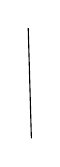
\begin{tikzpicture}\draw (0,0)--(.04,-1.4);\end{tikzpicture}}

\uline{Dém}\quad On peut supposer, par linéarité, que $A=\mathbb F_p$.
Mais c'est fait dans Demazure--Gabriel, II \S 3 4.6

\uline{Lemme 2}\quad Soit $H$ un sous-schéma en groupes de $G_a$, tel
\deleted{\unsure{fini}} que l'on ait $H\simeq G_a$, ou
\inserted{$H$ est fini loc. libre sur $S$,}
\deleted{\unsure{que $G/H$ est}}
$G/H$ est loc. isom. à $G_a$ (pour fppf).
Alors on a

a) $\underline{\operatorname{Ext}}^1(H,W_n)
\xrightarrow{R_*^{n-1}}\operatorname{Ext}^1(H,W_1)$ est bijection,

i.e. \deleted{$\unsure{V}\operatorname{Ext}^1(H,W_{n-1})
-\operatorname{Ext}^1(H,W_n)$ est nulle i.e.}
\deleted{$\unsure{\operatorname{Ext}}$}

\[
\begin{aligned}
a_1)\quad&
\operatorname{Ext}^1(H,W_{n-1})\xrightarrow{V}\operatorname{Ext}^1(H,W_n)
\quad\text{est nulle, i.e.}\\
&\operatorname{Hom}(H,G_a)-\operatorname{Ext}^1(H,W_{n-1})
\quad\text{est surjectif}\\
a_2)\quad&
\operatorname{Ext}^1(H,W_1)\longrightarrow\operatorname{Ext}^1(H,W_{n-1})
\quad\text{est nulle}
\end{aligned}
\]

b) $\operatorname{Ext}^1(G_a,W_n)-\operatorname{Ext}^1(H,W_n)$
\uline{surjective}

(i.e. $\operatorname{Ext}^1(H,W_n)-\operatorname{Ext}^2(G_a/H,W_n)$
est nulle)

c) $\underline{\operatorname{Ext}}^1(G_a,W_n)$ est un $A[F]$-module
\deleted{libre de base la}
\inserted{\uuline{à droite}, engendré par la}
classe \deleted{\unsure{e}} de $W_{n+1}$.

\uline{Dém}\quad \uline{$n=1$}\quad Alors a) est trivial,
b) résulte de $\underline{\operatorname{Ext}}^2(G_a/H,W_1)=0$
(qui résulte, par dévissage sur $n$ et descente fppf, de
$\underline{\operatorname{Ext}}^2(G_a,G_a)=0$)
et c) n'est autre que le lemme 1.

\inserted{\uline{$n$ général:}}
On procède comme dans \deleted{\unsure{le}} loc. cit.
\inserted{V \S 1 2.2.}, par récurrence sur $n$.
\margin{69}

\scanpage{60}
\uline{Corollaire 3}\quad Si $H$ est comme précédemment,
\unsure{on a} $\underline{\operatorname{Ext}}^1(H,\underline W)=0$
$(\underline W=\varinjlim_n W_n)$.
\figure{\begin{tikzpicture}\draw (0,0)--(0,-.5);\end{tikzpicture}}

\margin{\uline{Question} Si $S$ est affine, a-t-on
$\operatorname{Ext}^1(H,\underline W)=0$
i.e. $H^1(S,\underline{\operatorname{Hom}}(H,\underline W))=0$ ??
\uuline{Non} déjà pour $H=\alpha_p$, si $S=\operatorname{Spec}k$,
$k$ corps non parfait.}

\uline{Proposition 4} Soit $G$ un groupe algébrique
\deleted{\unsure{fini}} \inserted{fini, radiciel et unipotent}
sur un corps $k$ de car. $p>0$ \inserted{(pas néc. parfait)}
tel que $G$ soit annulé par $V^n$. Alors

\deleted{a) $\underline{\operatorname{Hom}}_{\mathrm{gp}}(G,W_n)$
est un schéma en groupes lisse \inserted{connexe}
\deleted{sur $k$ et dimension \unsure{$r=\dim G/G^0$}}
(et $\overline{\mathrm m}$ isomorphe à $\unsure{\mathbb E_k^r|\mathbb A_k^r}$
pour $r$ \deleted{$\unsure{\dim_k G}$}
$\operatorname{rg}G=p^r$)}

b) $\underline{\operatorname{Ext}}^1_{\unsure{\mathrm{gp}}}
(G,\underrightarrow W)=0$

Le b) provient du cor. 3, compte tenu que $G$ se dévisse en
groupes isom. à $\alpha_p$.

\deleted{Pour prouver a), on procède par récurrence sur la longueur
$r$ d'une \inserted{telle} suite de composition. On a donc
\[
0-G'\longrightarrow G-\alpha_p-0
\]
d'où une suite exacte
\[
0-\underline{\operatorname{Hom}}(\alpha_p,\underrightarrow W)
-\underline{\operatorname{Hom}}(G,\underline W)
-\underline{\operatorname{Hom}}(G',\underline W)\longrightarrow0
\]
compte tenu que $\underline{\operatorname{Ext}}^1(\alpha_p,\underline W)=0$.
Or les trois termes ne changent pas si on y remplace $\underline W$
par $W_n$. Enfin, on applique l'hyp. de récurrence à
$\underline{\operatorname{Hom}}(G',W_n)$, et on note que
$\underline{\operatorname{Hom}}(\alpha_p,W_n)\simeq G_a$.
On gagne!

5. Soit $\mathbb D(G)=\underline{\operatorname{Hom}}(G,\underrightarrow W)$.
C'est un $W_\infty$-Module, muni des endom $V$ et $F$ satisfaisant
les conditions habituelles (provenant des relations entre $V,F$
et les $\lambda\in W_\infty(S)$, qu'on a dans $\underrightarrow W$)
\[
(5.1)\qquad F\lambda=\lambda^{(p)}F,\quad
\lambda V=V\lambda^p,\qquad FV=VF=p.\operatorname{id}
\]
}
\margin{70}

\scanpage{61}
Groupes finis sur base de car. $p>0$.

\uline{Groupes finis étales}

Soit $G$ fini étale annulé par $p^n$. Pour tout épaississement
$S'$ de $S$, $G$ s'étend de façon unique en un groupe fini étale
$G'$ sur $S'$, également tué par $p^n$. Soit
$\mathcal M_{S'}=G'\otimes_{\mathbb Z/p^n\mathbb Z}
\underline{\mathcal O}_{S'}
=G'\otimes_{\mathbb Z/p^n\mathbb Z}
(\mathcal O_{S'}/p^n\mathcal O_{S'})$.
Pour $S'$ variable, on obtient un cristal $\mathbb D_*(G)$.
L'hom $G\xrightarrow{f}G^p$ est ici un isom. et définit un hom
\[
\unsure{F_*|F_\bullet}:\mathbb D_*(G)-\mathbb D_*(G)^{(p)}
\]
qui est un isomorphisme. Par dualité, posant
\[
\check G=\underline{\operatorname{Hom}}_{\mathrm{gr}}
(G,(\mathbb Q_p/\mathbb Z_p)_S),\qquad
\mathbb D^*(G)=\mathbb D_*(\check G)
\]
on trouve un \inserted{anti-}foncteur $G\longmapsto\mathbb D^*(G)$,
et
\[
F^*:\mathbb D^*(G)^{(p)}\xrightarrow{\sim}\mathbb D^*(G).
\]
$V^*$ est uniquement défini par $\deleted{\mathbb D^*(G)}$.
$F^*V^*=p\operatorname{id}_{\mathbb D^*(G)}$.

\deleted{\unsure{On} Dans la catégorie des cristaux de modules}

\uline{Cas}\quad $G$ \uline{plat sur} $\Lambda_n$
(i.e. groupe à B.T. tronqué d'échelon $n$).
Alors $\mathbb D^*(G)$ est un cristal de modules loc. libre de t.f.
rel. à $\Lambda_n$, \unsure{\&} avec $F$ \deleted{tel que}
un isomorphisme ($\mapsto V$ de façon unique) et on obtient une
\inserted{anti-}équivalence de la catégorie des
\deleted{\unsure{cris}} $G$ et des $F$-cristaux précédents.
\margin{\uline{vérifier}}
\figure{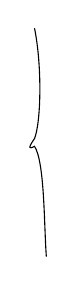
\begin{tikzpicture}
\draw (0,1.5) .. controls (.1,1) and (.08,.3) .. (0,.1)
.. controls (-.08,-.02) and (-.08,-.04) .. (0,0)
.. controls (.13,-.2) and (.12,-1) .. (.15,-1.4);
\end{tikzpicture}}

\uline{Cas général}\quad \inserted{Anti-}Équivalence entre la catégorie
des $G$, et celle des \inserted{$F$-}cristaux
(i.e. $F$-$V$-cristaux) sur $S$ qui loc. (ét) sont des sommes de
cristaux du type précédent (avec $n$ variable).

De ceci résulte que si $G\longleftrightarrow M$, on a
\[
G(S)\underset{\unsure{n\ \mathrm{grd.}}}{\simeq}
\operatorname{Hom}_{\mathrm{gr}}(\Lambda_{nS},G)
\simeq\operatorname{Hom}_{F-V-\mathrm{cris}}
(M,\mathcal O_{S,n\,\mathrm{cris}})
\simeq\operatorname{Hom}_{F-\mathrm{cris}}(\unsure{-})
\]
\margin{71}

\scanpage{62}
Comme $\ell_\bullet^G=0$, le triangle exact de dualité pour $G$
se réduit à
\diagram{\begin{tikzcd}[ampersand replacement=\&,column sep=small,row sep=small]
\&\check\ell_\bullet^{G^*}[1]\arrow[dl]\&\\
0\arrow[rr,no head]\&\&\Delta_\bullet(G)\arrow[ul,"\unsure{\sim|2}"']
\end{tikzcd}}
i.e. ne donne pas de structure supplémentaire
\deleted{\unsure{rel. à} $\unsure{G}$} \inserted{en sus}
du cristal $M$. On a
\[
\begin{aligned}
\check\ell_\bullet^{G^*}[1]
&\simeq\unsure{\underline{\Sigma}^*(G)|\underline{\mathbb D}^*(G)}
\simeq\varepsilon^*(M_{/p})
=\deleted{\unsure{\varepsilon}}
R\underline{\operatorname{Hom}}_{\mathbb Z}(G,\underline{\mathcal O}_S)\\
&\simeq\check G\overset L\otimes_{\mathbb Z}\underline{\mathcal O}_S
\simeq(\check G\overset L\otimes_{\mathbb Z}\mathbb F_p)
\otimes_{\mathbb F_p}\underline{\mathcal O}_S.
\end{aligned}
\]

\uline{Groupes de type multiplicatif}
(\unsure{annulés} par puiss. $p^n$ de $p$)

Soit $G$ \deleted{est} un tel, il est défini par $G^*$,
groupe étale annulé par $p^n$, auquel s'appliquent les réflexions
précédentes. On aura
\[
\mathbb D^*(G)=\mathbb D_*(G^*)
\]
i.e.
\[
\mathbb D^*(G)_{S'}=(G^*_{S'})\otimes_{\mathbb Z_p}
\underline{\mathcal O}_{S'}
\]
\inserted{$G^*_{S'}$: groupe étale sur $S'$ prolongeant $G^*$}

Ici
\[
V:\mathbb D^*(G)\longrightarrow\mathbb D^*(G^{(p)})
=\mathbb D^*(G)^{(p)}
\]
est un isomorphisme, savoir
$\mathbb D_*(f_{G^*}:G^*\longrightarrow G^{*(p)})$,
et $F$ est \inserted{par suite} déterminé uniquement en termes de $V$.

On a encore des équivalences de catégories
\diagram{\[\begin{array}{ccl}
\text{groupes de B.T. tronqués d'échelon }n\text{ de t.m.}
&\simeq&
\text{cristaux loc. libres de t.f.}\\
&&\text{pour }S/\Lambda_n,\text{ avec }V\\
&&\text{un isom (et }F\text{ si on veut)}
\end{array}\]}
\margin{72}

\scanpage{63}
et équivalences analogues pour les groupes
\deleted{de B.T. \unsure{de}} de type multiplicatif annulés par une
puissance de $p$. \deleted{On constate encore}
Ici $\check\ell_\bullet^{G^*}[1]=0$, et le triangle exact de dualité
se réduit à
\diagram{\begin{tikzcd}[ampersand replacement=\&,column sep=small,row sep=small]
\&0\arrow[dl]\&\\
\ell_\bullet^G\arrow[rr]\&\&\Delta_\bullet(G)\arrow[ul]
\end{tikzcd}},
avec $\ell_\bullet^G$ donné comme dessus
\[
\ell_\bullet^G\simeq G^*\overset L\otimes_{\mathbb Z}
\underline{\mathcal O}_S
\simeq(G^*\overset L\otimes_{\mathbb Z}\mathbb F_p)
\otimes_{\mathbb F_p}\underline{\mathcal O}_S.
\]

\uline{Homomorphismes entre groupes étales et groupes de} t.m.
\deleted{\unsure{tronqués}}

a) Un hom d'un groupe de t.m. $G$ dans un étale $G'$ est nul.
D'autre part, tout \deleted{$\unsure{F}$} hom \inserted{$u$} de
$F$-$V$-cristaux (ou simplement de $F$-cristaux, ou de $V$-cristaux)
de $M'$ dans $M$ est nul.
En effet, écrivons la commutativité à $F^n$ pour $n$ assez grand,
en notant que $F_{M'}^n$ est un isom et $F_M^n$ est nul
(pour $n$ grand), d'où \unsure{aussitôt} le résultat pour les $F$-hom,
et on procède de $\overline{\mathrm m}$ pour les $V$-hom.

b) Hom. d'un groupe étale $G$ dans un groupe de t.m. $G'$.
\margin{73}

\scanpage{65}
$S$ schéma de car $p$.

$\mathcal C$ catégorie des schémas en groupes finis étales
\inserted{$E$} sur $S$ annulés par $p$
$\simeq$ catégorie des faisceaux \unsure{étales}
$\mathbb F_p$-vectoriels loc. libres de type fini.

$\mathcal C'$ catégorie des Modules loc. libres $M$ sur $S$, munis de
\[
F_M:M^{(p)}\xrightarrow{\sim}M.
\]
\[
\mathcal C\xrightarrow{\varphi}\mathcal C',
\qquad E\longmapsto
(E\otimes_{\mathbb F_p}\underline{\mathcal O}_S,
F_E\otimes_{\mathbb F_p}\underline{\mathcal O}_S)
\]
\[
\uline{\text{NB}}\quad
(E\otimes_{\mathbb F_p}\underline{\mathcal O}_S)^{(p)}
\simeq E^{(p)}\otimes_{\mathbb F_p}\underline{\mathcal O}_S
\xleftarrow[\unsure{f_{E/S}}]{\sim}
E\otimes_{\mathbb F_p}\underline{\mathcal O}_S)
\]

\uline{Proposition}\quad \uline{Le foncteur} $\varphi$
\uline{est une équivalence de catégories}.

a) \uline{Pleinement fidèle}. \deleted{\unsure{P}}
Par passage à des \uline{Hom}, revient à ceci:
\[
\Gamma(S,E)\xrightarrow{\sim}
\{x\in\Gamma(S,E\otimes_{\mathbb F_p}\mathcal O_S)
\mid F(x^{(p)})=x\}
\]
Par descente, on se ramène au cas $E$ constant, puis
$E=\mathbb F_{pS}$, et on est ramené alors à l'assertion que
\[
0-(\mathbb Z/p\mathbb Z)_S-G_{aS}
\xrightarrow{x\mapsto x^p-x}G_{aS}
\]
est exacte, ce qui est bien connu (il suffit de le voir sur
$\mathbb F_p$ par chgt de base \dots).

b) Essentiellement surjectif. Si $(M,F)$ est donné, il suffit
de voir qu'il est \uline{loc} de la forme voulue.
Considérons
\[
M\xrightarrow{\inserted{\unsure{\delta x}=F_Mf_Mx-x}}M
\]
on voit que c'est un \deleted{\unsure{iso}}morphisme étale de
schémas en groupes, donc son noyau est un schéma en groupes étale
$E$ sur $S$. Pour montrer qu'il est fini sur $S$, il suffit de
prouver qu'il est de \inserted{$\mathbb F_p$-}rang
\deleted{\unsure{égal}} \unsure{localt ct} \unsure{et un}
fini, égal au rang de $M$. Pour prouver ensuite que
$E\otimes_{\mathbb F_p}\mathcal O_S-M$ est un isom, il suffit de
le prouver fibre par fibre (géom). Bref, on est ramené au cas
\margin{75}

\scanpage{66}
d'un corps de base alg. clos, et à prouver donc:

\uline{Lemme}\quad Soit $M$ vectoriel sur $k$
\deleted{\unsure{parf.}}\inserted{alg.} clos de car $p$,
muni de $F_M:M^{(p)}\xrightarrow{\sim}M$.
Soit $E=\{x\in M,\ Fx^{(p)}=x\}$. Alors
$E\otimes_{\mathbb F_p}k\xrightarrow{\sim}M$.
\figure{\begin{tikzpicture}\draw (0,0)--(0,-.7);\end{tikzpicture}}

\figure{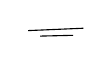
\begin{tikzpicture}
\draw (0,0)--(.7,.03); \draw (.15,-.07)--(.57,-.06);
\end{tikzpicture}}

$\mathcal C$ catégorie des schémas en \inserted{$p$-}groupes
\deleted{\unsure{finis et étales}} \inserted{finis étales} sur $S$
\inserted{i.e. des faisceaux en $p$-groupes loc. constants de t.f.}
\deleted{\unsure{catégorie des schémas}}

$\mathcal C'$ catégorie des \deleted{schémas}
\inserted{faisceaux} en $W_S^{\unsure{\mathrm{can}}}$-modules $M$
loc. isom à une somme de copies de $W_{nS}$, munis
$\deleted{\unsure{de}}\ M^{(p)}\xrightarrow[\sim]{F_M}M$.
\margin{Zar ou fppf, c'est \unsure{kif kif}}
\figure{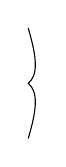
\begin{tikzpicture}
\draw (0,.7)..controls(.12,.3)and(.12,.1)..(0,0)
..controls(.12,-.1)and(.12,-.3)..(0,-.7);
\end{tikzpicture}}

$\mathcal C''$ catégorie des schémas en $W_S$-modules lisses

\diagram{\begin{tikzcd}[ampersand replacement=\&]
\mathcal C\arrow[r,"\varphi"]\arrow[dr,"\psi"']\&
\mathcal C'\arrow[d,"i\ \unsure{\sim}"]\\
\&\mathcal C''
\end{tikzcd}}

$\varphi(E)=E\otimes_{\mathbb Z_p}W_S^{\unsure{\mathrm{can}}}$
avec le $F$ qu'on devine

$i(M)=$ \deleted{faisceau en groupes}
\inserted{schéma} représentant le faisceau\dots

$\psi(E)=E\otimes_{\mathbb Z_p}W_S$
\margin{76}

\scanpage{67}
\begin{tabular}{c}
\textbf{COLLÈGE}\\[.3em]
\textbf{DE}\\[.3em]
\textbf{FRANCE}\\
---
\end{tabular}
\hfill\textit{Paris, le}

\margin{\unsure{EUX}\quad\unsure{OCF}\quad SAVOYEUX\quad\unsure{O}}
\margin{77}

\cotefile{7}
\scanpage{1}
\figure{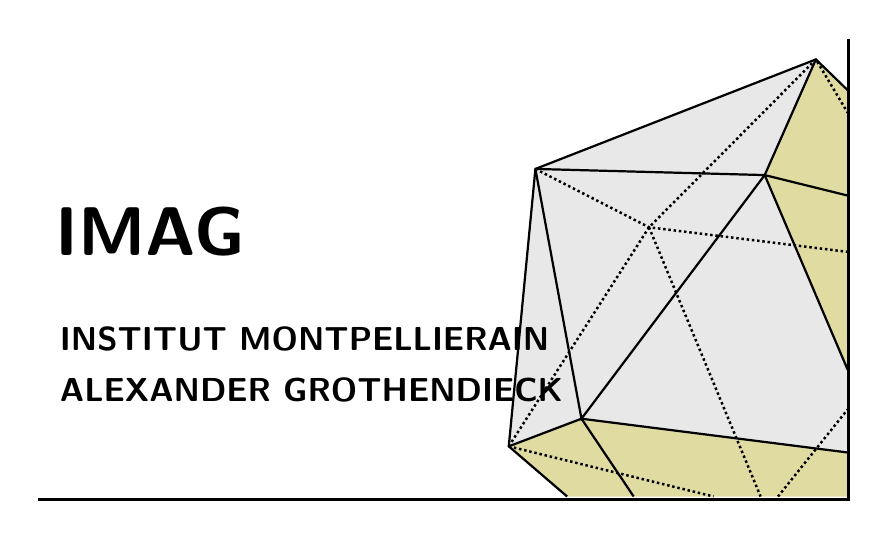
\begin{tikzpicture}[x=.013cm,y=-.013cm]
\clip (0,0) rectangle (806,466);
\fill[gray!18] (496,138)--(770,31)--(720,144)--(801,334)--(801,415)--(541,382)--(470,409)--cycle;
\fill[olive!28] (770,31)--(801,61)--(801,334)--(720,144)--cycle;
\fill[olive!28] (470,409)--(541,382)--(801,415)--(801,458)--(527,458)--cycle;
\draw[line width=.8pt] (496,138)--(770,31)--(801,61);
\draw[line width=.8pt] (770,31)--(720,144)--(496,138)--(470,409)--(527,458);
\draw[line width=.8pt] (496,138)--(541,382)--(720,144)--(801,164);
\draw[line width=.8pt] (720,144)--(801,334);
\draw[line width=.8pt] (470,409)--(541,382)--(801,415);
\draw[line width=.8pt] (541,382)--(592,458);
\draw[densely dotted,line width=.9pt] (496,138)--(607,195)--(801,219);
\draw[densely dotted,line width=.9pt] (470,409)--(607,195)--(770,31)--(801,83);
\draw[densely dotted,line width=.9pt] (607,195)--(716,458);
\draw[densely dotted,line width=.9pt] (470,409)--(670,458);
\draw[densely dotted,line width=.9pt] (733,458)--(801,373);
\draw[line width=1.3pt] (10,461)--(802,461)--(802,11);
\node[anchor=west,font=\sffamily\bfseries\fontsize{64}{66}\selectfont]
at (18,199) {IMAG};
\node[anchor=west,font=\sffamily\bfseries\fontsize{12}{14}\selectfont]
at (22,304) {INSTITUT MONTPELLIERAIN};
\node[anchor=west,font=\sffamily\bfseries\fontsize{12}{14}\selectfont]
at (22,354) {ALEXANDER GROTHENDIECK};
\end{tikzpicture}}

\scanpage{3}
\margin{Juillet--Août \unsure{1967}}

Anneaux \deleted{\unsure{semi-}}simpliciaux canoniques et modules
stratifiés. \deleted{\unsure{cristaux}}
[Formellement, les développements qui suivent sont indépendants
des \deleted{\unsure{crist.}} histoires de Sites cristallins ou
\unsure{Antipiants|stratifiants}].

1. Soit $X\longrightarrow S$ un préschéma relatif.
Pour tout entier $n\geq0$, soit
\[
X^{[n]}=\underbrace{X\times_S\cdots\times_S X}_{n+1}
\]
considéré comme objet \deleted{de $\unsure{X/(\mathrm{Sch}/S)}$}
de $(\mathrm{Sch})_{/S}$, muni de \deleted{\unsure{diag}}
l'immersion
$X\xrightarrow{\operatorname{diag}_n}X^{[n]}$.
Soit $X^{\widehat{[n]}}$ son complété formel le long de $X$.
Pour $n\geq0$ variable, on trouve un objet simplicial à valeurs
dans $\mathrm{Schf}/X$, les espaces sous-jacents aux
$X^{\widehat{[n]}}$ étant d'ailleurs tous égaux à $\operatorname{esp}(X)$.

Soit $\mathcal P^n$
$\deleted{\unsure{\mathcal O_{X^{\widehat{[n]}}}}}$
le faisceau structural de $X^{\widehat{[n]}}$,
\deleted{\unsure{vu dans}} considéré comme
\deleted{\unsure{anneau}}
\inserted{$\mathbb N$-pro-objet de \unsure{la}}
la catégorie des faisceaux d'anneaux sur $\operatorname{esp}(X)$,
i.e. dans $\operatorname{Pro}(\operatorname{Ann}(\operatorname{esp}(X)))$.
Pour $n$ variable, on trouve ainsi un Anneau cosimplicial
$\mathcal P^*$ sur $\operatorname{esp}(X)$, avec
$\mathcal P^0=\underline{\mathcal O}_X$.
Faire attention que ce \uline{n'est}
\margin{2}

\scanpage{4}
\uline{pas} une $\mathcal O_X$-Algèbre cosimpliciale, car les deux hom
$\mathcal O_X=\mathcal P^{[0]}\rightrightarrows\mathcal P^{[1]}$
sont en général distincts, et \unsure{mettent} sur $\mathcal P^{[1]}$
deux structures \uline{distinctes} de $\mathcal O_X$-algèbres.

Considérons l'objet shifté $S\mathcal P$, défini par
\[
(S\mathcal P)^i=\mathcal P^{i+1}
\]
ou fonctoriellement par
\[
(S\mathcal P)(I)=\mathcal P(I\amalg e)
\]
$e$ un ensemble réduit à un élément.
L'hom \inserted{fonctoriel} $I-I\amalg e$ définit
$\mathcal P(I)\longrightarrow\mathcal P(I\amalg e)$ i.e.
\[
\alpha^*:\mathcal P^*\longrightarrow(S\mathcal P)^*
\qquad\text{i.e. }\alpha^i:\mathcal P^i-\mathcal P^{i+1}
\]

Si p.ex. $S=\operatorname{Spec}k$ ($k$ un anneau),
$X=\operatorname{Spec}A$, $X$ étant tel que $X-X\times_SX$
soit une nil-immersion [p.ex. $X$ radiciel de t.f. sur $S$]
alors \inserted{passant aux sections}
\[
\Gamma\mathcal P^i=\bigotimes_k^{i+1}A
=\underbrace{A\otimes_k A\otimes\cdots\otimes_k A}_{i+1}
\]
les op. simpliciales sont celles qu'on devine, et l'hom $\alpha$
étant donné par
\[
\underbrace{A\otimes\cdots\otimes A}_{i+1}
\longrightarrow\underbrace{A\otimes\cdots\otimes A}_{i+2}
\]
\[
\alpha^i(a_0\unsure{-\cdots-}x_i)
=a_0\otimes\cdots\otimes a_i\otimes1
\]
\margin{3}

\scanpage{5}
2. Soit $\deleted{(}M\deleted{,\unsure{\varepsilon_M})}$ un Module sur $X$. \deleted{stratifié} \deleted{rel. à $S$.} On pose pour $i\geq0$
\[
\mathcal P^i[M]=\mathcal P^{i\deleted{\unsure{*}}}\otimes_{\underline O_X}M
\]
où $\mathcal P^{i\deleted{\unsure{*}}}$ est considéré comme Algèbre sur $\underline O_X$ par sa structure \uline{extrême-droite}. \deleted{\unsure{Donc} $\mathcal P^i(M)$ est un} Par définition, le produit tensoriel doit être interprété comme un pro-objet [tout comme $\mathcal P^i$] --- ce n'est que sous des conditions exceptionnelles [p.ex $M$ libre de type fini, $X$ \inserted{loc} noeth, \deleted{\unsure{$S$}} $\Omega_{X/S}$ \unsure{coh} et $M$ de type fini sur $X$] que l'on est justifié d'interpréter $\mathcal P^i\deleted{\unsure{[\,]}}$ et $\mathcal P^i[M]$ comme des faisceaux au lieu de profaisceaux. [car dans ces cas, on récupère les profaisceaux à partir des \deleted{\unsure{leurs}} $\varprojlim$]. On notera que $\mathcal P^i(M)$ est un $\mathcal P^i$-Module, dépendant fonctoriellement de $M$ variable \unsure{de|dans} $\operatorname{Mod}(\underline O_X)$.
Si on prend comme hom de $M$ en $N$
\margin{4}

\scanpage{6}
de $\underline O_X$ sur les $Q^i=\mathcal P^{i+1}$ \unsure{commutent} à cette structure. Il s'ensuit que les
$Q^i[M]=\underset{\inserted{\text{[str. ext. dr.]}}}{Q^i}\otimes_{\underline O_X}M$
sont les composantes d'un objet \deleted{\unsure{semi-}}cosimplicial, noté $Q^*[M]$, qui est en fait un \uline{Module} cosimplicial sur l'anneau cosimplicial $\mathcal P^*$.
Ce $Q^*[M]$ dépend également de façon fonctorielle de $M$, quand $M$ parcourt $\operatorname{Mod}(X/S)$.

3. Notons un caractère hautement spécial des Modules cosimpliciaux de la forme $Q^*[M]$ sur $\mathcal P^*$ : \deleted{ils} \deleted{\unsure{sont des}} c'est que les $Q^i[M]$ se déduisent les uns des autres par changement de base via les opérations simpliciales $\mathcal P^i\longrightarrow\mathcal P^j$ [i.e. ce sont des \deleted{\unsure{petits}} objets d'un $\varprojlim$, non seulement
\margin{5}

\scanpage{7}
d'un $\unsure{\underline\Gamma}$]. Formellement, [de façon précise : à cela près qu'on a des pro-Modules au lieu de Modules tt courts] on voit que $Q^0[M]$ est un (pro)Module stratifié sur $X$ rel $S$, et les $Q^i[M]$ sont les composantes du (pro)Module \deleted{\unsure{$Q$}} cosimplicial correspondant.
\margin{\figure{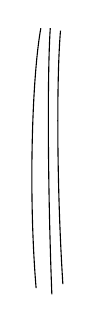
\begin{tikzpicture}[x=1cm,y=1cm]
\draw (0,0) .. controls (-.10,1.2) and (-.05,2.7) .. (.06,3.3);
\draw (.20,-.08) .. controls (.15,1.2) and (.14,2.7) .. (.18,3.3);
\draw (.34,.05) .. controls (.26,1.3) and (.26,2.7) .. (.31,3.27);
\end{tikzpicture}}}

Ce pro-Module stratifié $Q^0[M]$, \inserted{des parties principales} dépend fonctoriellement de $M$ parcourant $\operatorname{Mod}(X/S)$ [Modules sur $X$ avec op. diff. \inserted{rel $S$} d'\uline{\deleted{\unsure{un}}\inserted{ordre} borné}], en prenant comme hom de pro-objets ceux au sens de Artin-Riesz.
De plus, on récupère $M$ à partir de $Q^0[M]$ [pro-objet à stratification] comme étant le sous-faisceau des \uline{sections stationnaires} [\unsure{dans la structure}
\margin{\figure{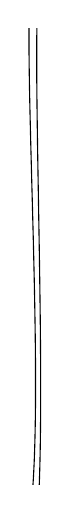
\begin{tikzpicture}[x=1cm,y=1cm]
\draw (0,0) .. controls (.10,1.5) and (-.06,4.4) .. (-.05,5.8);
\draw (.08,0) .. controls (.14,1.6) and (.03,4.5) .. (.05,5.8);
\end{tikzpicture}}}
\margin{6}

\scanpage{8}
de $\underline O_X$-Module provenant de l'extrême droite
[NB. les structures extrême-droites des $Q^i[M]$ sont compatibles avec les op. simpliciales, i.e. $Q^{\unsure{i}}[M]$ est un Module cosimplicial à $\underline O_X$ opérant par ses op. extrême-droites ; mais bien sûr cette dernière structure n'est pas conservée par les hom $M-N$ qui sont non $\underline O_X$-lin (mais seult des op. diff. rel / $S$)]. De $\overline{\mathrm m}$, un hom $D:M-N$ de $\operatorname{Mod}(X/S)$ est récupéré à partir de $Q^0[D]:Q^0[M]\unsure{-|\longrightarrow}Q^0[N]$ comme l'hom induit sur les ss-faisceaux des \deleted{\unsure{objets}}\inserted{sections} stationnaires.

4. Une façon équivalente d'obtenir $Q^*[M]$ est de considérer
\diagram{\begin{tikzcd}[ampersand replacement=\&,column sep=large]
X^{\widehat{[2]}}\arrow[r,shift left=.7ex]\arrow[r,shift right=.7ex]\&X^{\widehat{[1]}}\arrow[r,"\widehat{\operatorname{pr}}_2"]\&X^{\widehat{[0]}}=X
\end{tikzcd}}
et les produits fibrés [dans la cat. des présch. formels sur $X$], \deleted{\unsure{donc}} c'est aussi
\margin{7}

\scanpage{9}
qu'on trouve l'anneau \inserted{cosimplicial} $Q^*$, et $Q^*[M]=Q^*\otimes_{\underline O_X}M$. Comme $X^{\widehat{[1]}}$ a une section sur $X^{\widehat{[0]}}$, on obtient aussitôt que \uline{$Q^*[M]$ est une résolution de} $M$ [en mettant sur ts les $Q^i[M]$ les structures extrême-droites de $\underline O_X$-Modules]. Il faut cependant préciser le sens qu'on attache à cette expression [les A.R.-pro-modules forment-ils une catégorie abélienne ?....] et s'assurer s'il ne faut pas une hypothèse de quasi-cohérence sur $M$.
En tous cas, \deleted{\unsure{pour}} \unsure{dénotant|désignant} par un $\ell$ le passage aux $\varprojlim$ des pro-objets, on trouve que $\ell Q^*[M]$ est une résolution de $M$ si $M$ \unsure{qu coh.}
\margin{8}

\scanpage{10}
et par suite on trouve en tous cas
\diagram{\begin{tikzcd}[ampersand replacement=\&,column sep=small,row sep=large]
H^*(X,M)\simeq\&\mathbb H^*(X,\ell Q^*[M])\\
\&E_2^{pq}=H^p(i\mapsto H^q(X,\ell Q^i[M])\arrow[u,Rightarrow]
\end{tikzcd}}

[Sous des conditions convenables, on aura
\[
H^q(X,\ell Q^i[M])=\varprojlim_n H^q(X,Q^i_{\deleted{\unsure{n}}}[M]_{(n)})
\deleted{\unsure{\simeq H^q(X^{\widehat{[i]}},M)}}
\inserted{\simeq H^q(X_{\unsure{n|x}}^{\widehat{[i+1]}},M)}
\]
\margin{\figure{\begin{tikzpicture}[x=1cm,y=1cm]
\node at (0,2.3) {\unsure{Attention}};
\node at (-.7,1.8) {$-$};
\node[draw,ellipse,inner sep=2pt] at (0,1.8) {$+1$};
\node at (0,1.25) {\unsure{nom de|au lieu de} $\widehat{\ }$ !};
\draw (-1.2,.75) .. controls (1.8,.3) and (1.6,2.9) .. (0,2.8) .. controls (-.6,2.8) and (-1,2.65) .. (-1.25,2.55);
\node at (0,.4) {$X^{[i+1]}=[X/S]^{i+2}$};
\node at (0,-.1) {($i+2$ facteurs !)};
\end{tikzpicture}}}
si on écrit
\[
\begin{aligned}
Q^i[M]&=\varprojlim_n Q^i[M]_{(n)}\\
Q^i[M]_{(n)}&=Q^i_{(n)}\otimes_{\underline O_X}M\\
Q^i_{(n)}&=\mathcal P^{\unsure{i+1}}_{(n)}=\cdots
\end{aligned}
\]
].

Si on remplace $M^{\unsure{2|*}}$ par un \uline{complexe} $M^\bullet$ de \deleted{\unsure{$C$}} $D^+(\operatorname{Mod}(X/S))=D^+(X/S)$, on obtient un bicomplexe $Q^*[M^\bullet]$, tel que $\ell Q^*[M^\bullet]$ est une résolution de $M^\bullet$, et par suite
\[
H^*(X,M)\simeq H^*(X,Q^*[M^\bullet])\simeq H^*(X_{\unsure{\mathrm{str}}},\unsure{Q^0(M^\bullet)})
\]
[$Q^0[M^\bullet]$ s'appelle la \uline{\unsure{formalisation}} du complexe \deleted{\illegible{1}} d'op. différentielles $M$.
\margin{\figure{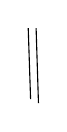
\begin{tikzpicture}[x=1cm,y=1cm]
\draw (0,0)--(-.03,.9);
\draw (.10,-.05)--(.07,.9);
\end{tikzpicture}}}
\margin{9}

\scanpage{11}
5. Soit tjrs $M^\bullet\in\operatorname{Ob}D^+(X/S)$, et considérons le complexe $Q^0[M^\bullet]$ \deleted{de} \deleted{\unsure{de $Q^0[$}} de (pro-$\underline O_X$-Modules) à stratification, dont la connaissance implique celle de $M^\bullet$ : du pt de vue de \unsure{complexe} additif d'abord, en passant aux faisceaux des sections stationnaires, puis les $\underline O_X$-structures sur les $M^i$ comme restrictions des structures extrême-droites des $Q^0[M^i]$ (lesquelles, rappelons le encore, ne sont cependant pas respectées par l'op. diff. de $Q^0[M^\bullet]$).

Considérons les $\mathcal H^i(\ell Q^0[M^\bullet])$, et supposons que leur formation commute aux changts de base \deleted{\unsure{semi}}\inserted{co}-simpliciaux $\mathcal P^0\longrightarrow\mathcal P^{\deleted{\unsure{1}}n}$ ; ceci sera assuré par des hypothèses
\margin{10}

\scanpage{12}
de \inserted{\unsure{hypo}} platitude sur les $Q^0[M^\bullet]$ et les $\mathcal H^i(Q^0(M^\bullet))$, \deleted{\unsure{qui en sont}} soit (plus économiques, sans doute, vu que l'on ne peut guère avoir de platitude sur $\underline O_X$ de $Q^0[M^\bullet]$ sans celle de $X^{\widehat{[1]}}\unsure{-|\longrightarrow}X^0$\unsure{]|)} une hypothèse de ``\uline{platitude infinitésimale de} $X/S$'' i.e. \inserted{une hypo. de \deleted{\unsure{pro}} platitude sur} $X^{\widehat{[1]}}\unsure{-|\longrightarrow}X$ --- p.ex. $X/S$ plat
\[
\cdots\quad[\text{critères : dégager}].
\]
Alors
\margin{\figure{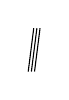
\begin{tikzpicture}[x=1cm,y=1cm]
\draw (0,0)--(.07,.55);\draw (.04,0)--(.11,.55);\draw (.08,0)--(.15,.55);
\end{tikzpicture}}}
\deleted{\unsure{(a)}} $1^\circ)$ Les $V^i=\mathcal H^i(\ell Q^0[M])$ sont de façon naturelle des $\underline O_X$-Modules (par la \inserted{$\underline O_X$-}structure gauche) \uline{stratifiés}.

$2^\circ)$ Dans le bicomplexe $\ell Q^*[M^\bullet]$, prenant les \inserted{faisceaux de} cohomologie suivant l'op. diff. provenant de $M^\bullet$ nous donne précisément les \deleted{\unsure{$Q$}} complexes $C^\bullet(V^i)$ attachés aux \deleted{connexions}\inserted{stratifications} des $V^i$.

$3^\circ)$ Par suite, on trouve une suite spectrale
\margin{11}

\scanpage{13}
\diagram{\begin{tikzcd}[ampersand replacement=\&,column sep=small]
\mathbb H^*(X,M^\bullet)\simeq\mathbb H^*(X,Q^*[M^\bullet])\&
E_2^{pq}=\mathbb H^p(X,C^\bullet(V^q))\arrow[l,Rightarrow]
\end{tikzcd}}
(\unsure{réf} à EGA $\underline O_{\mathrm{III}}$ ?). On peut encore l'écrire, en posant par définition, pour un Module stratifié $\underline{\unsure{V}}$ relativement à $S$,
\[
H^p(X_{\inserted{\mathrm{str}}}\deleted{\unsure{/S}},\underline V)
=\mathbb H^p(X,C^\bullet_{\mathrm{str}}(\underline V)),
\]
sous la forme
\diagram{\[\boxed{\begin{gathered}
\begin{tikzcd}[ampersand replacement=\&,column sep=small]
\mathbb H^*(X,M^\bullet)\&E_2^{pq}=H^p_{\deleted{\unsure{\mathrm{str}}}}(X_{\inserted{\mathrm{str}}},V^q(M^\bullet))\arrow[l,Rightarrow]
\end{tikzcd}\\[1em]
\text{où}\qquad V^q(M^\bullet)=\mathcal H^q(Q^0[M^\bullet])
\end{gathered}}\]}

\uline{Corollaire} Supposons que l'on ait
\[
V^q(M^\bullet)=0\quad\text{pour}\quad q\neq q_0
\]
alors on a des isom canoniques
\[
\mathbb H^n(X,M^\bullet)\simeq H^{n-q_0}_{\mathrm{str}}(X,V^{q_0}(M^\bullet))
\]
\margin{\figure{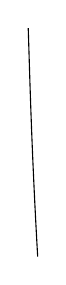
\begin{tikzpicture}[x=1cm,y=1cm]
\draw (0,0) .. controls (-.08,1.4) and (-.1,2.3) .. (-.12,2.9);
\end{tikzpicture}}}
Ceci montre, \inserted{supposant p.ex. que $q_0=0$,} que le premier \unsure{mb}
\margin{12}

\scanpage{14}
ne dépend que du Module stratifié $\underline V=V^{q_0}(M^\bullet)$ et de \deleted{\unsure{$q_0$}} $q_0$, mais pas du complexe différentiel particulier choisi pour ``résoudre'' $\underline V$.

6. Or, \deleted{\unsure{si $X$ est lisse sur $S$} \uline{\unsure{et de}} \uline{\unsure{car. $0$}} \unsure{(absolue)}} si on part d'un Module stratifié $\underline V$ sur $X$ rel / $S$, on peut tjrs lui associer de façon naturelle un \uline{complexe de De Rham}, dont l'objet gradué sous-jacent est
\[
\underline\Omega^\bullet_{X/S}\otimes\underline V=\Omega^\bullet(\underline V),
\]
et on vérifie, \uline{lorsque} \inserted{$X$ est lisse sur $S$ et,} \uline{$S$ est de car. nulle}, que ce complexe est bien une ``résolution différentielle'' de $\underline V$.
\margin{\figure{\begin{tikzpicture}
\node[draw,ellipse,rotate=25,align=center,inner sep=3pt] {``Lemme de\\Poincaré formel''};
\draw (-.8,.4)--(-.8,1.1);\draw (-.73,.4)--(-.73,1.1);\draw (-.66,.4)--(-.66,1.1);
\end{tikzpicture}}}
Dans ce cas, on trouve donc une interprétation \unsure{univoque} de la
\margin{\figure{\begin{tikzpicture}
\node[draw,ellipse,inner sep=4pt] {\unsure{différentielles|différentielle}};
\end{tikzpicture}}}
\margin{13}

\scanpage{15}
coh. de De Rham de $X/S$
\[
H^*_{\mathrm{DR}}(X/S,\underline V)\simeq H^*_{\mathrm{str}}(X/S,\underline V)
\]
au second mb duquel il n'est plus question de \deleted{cohomologie} formes différentielles !

Si on ne fait plus d'hyp. de lissité ni de caractéristique, il reste vrai qu'on a un hom canonique \inserted{compatible aux stratifications}
\diagram{\begin{tikzcd}[ampersand replacement=\&]
\underline V\arrow[r]\&\mathcal H^0(\ell Q^0[\Omega^\bullet(V)])
\end{tikzcd}}
i.e. un hom de complexes de Modules stratifiés
\diagram{\begin{tikzcd}[ampersand replacement=\&]
\underline V\arrow[r]\&\deleted{\unsure{\ell}}Q^0[\Omega^\bullet(V)]
\end{tikzcd}}
d'où en passant aux $C^\bullet_{\mathrm{str}}$ des deux \unsure{mbs}, un \uline{hom. can.}
\diagram{\[\boxed{\begin{tikzcd}[ampersand replacement=\&,column sep=large]
H^*(X_{\inserted{\mathrm{str}}}\deleted{\unsure{/S}},\underline V)\arrow[r]\&H^*_{\mathrm{DR}}(X/S,\underline V)
\end{tikzcd}}\]}
\margin{14}

\scanpage{16}
qui est donc un isom si $X/S$ est eff\textsuperscript{t} lisse et $S$ de car. nulle.

Je doute que ce soit tjrs un isom, \inserted{$\overline{\mathrm m}$} si $X$ est \uline{lisse et projectif} \inserted{(p.ex. une variété elliptique)} sur $S$ spectre d'un corps (alg. clos si on veut) de car $p>0$ ; \inserted{et $\underline V=\underline O_X$ avec stratification canonique.} Dans ce cas particulier, il n'est pas $\overline{\mathrm m}$ clair à priori que les $H^i_{\mathrm{str}}$ soient de dim finie, ni qu'ils soient nuls pour $i$ grand.
\uline{Situation à éclaircir !}
\margin{\figure{\begin{tikzpicture}[x=1cm,y=1cm]
\draw (1.6,6) ellipse (.53 and .37);
\draw (1.2,5.75) .. controls (-.2,4.6) and (-.7,4.8) .. (-.6,3.5) .. controls (-.6,2.9) and (-.2,2.6) .. (-.25,2.25);
\node[draw,ellipse,align=center,rotate=30,inner sep=3pt] at (0,1.65) {C'est en\\effet faux !};
\node[draw,align=center,rotate=30,inner sep=4pt] at (0,.15) {(\unsure{Calculs très}\\\unsure{amusants} pour\\$X/S$ \unsure{elliptique} ou\\abélien !)};
\draw (-.65,2.1)--(-.65,2.7);\draw (-.58,2.1)--(-.58,2.7);\draw (-.51,2.1)--(-.51,2.7);
\end{tikzpicture}}}

\uline{Remarque} L'intérêt de relier la coh. de De Rham à la cohomologie \deleted{\unsure{au sens}} $H_{\mathrm{str}}$ est que celle-ci, à son tour, s'interprète comme la cohomologie d'un ``site stratifiant'' convenable, dont une variante \unsure{ce|ns} \unsure{conduira} à la ``coh. $p$-adique en car. $p$''.
\margin{15}

\scanpage{17}
\S--- \uline{Commentaires sur la définition d'une cohomologie $p$-adique en car. $p>0$}

$X_0$ schéma sur corps parfait $k$ de car. $p>0$, $S=\unsure{\operatorname{Spec}|\operatorname{Spf}}W(k)$. Alors
\[
H^*(X_0/S,\mathrm{cris};\underline O_{X_0\,\mathrm{cris}})
\]
est un $W$-module gradué. \deleted{\unsure{L'espoir}} Mon espoir initial était qu'il soit \deleted{un} ``le'' bon candidat pour une cohomologie $p$-adique. Un premier \unsure{support} \deleted{\unsure{(moral)}} en faveur, c'est que lorsque $X_0$ \inserted{est lisse sur $k$, et pour simplifier,} se remonte en $X$ \deleted{propre et}\inserted{projectif et} lisse sur $\unsure{k|W}$, alors d'après l'exposé précédent, on trouve aisément
\[
H^*((X_0\deleted{\unsure{/S}})_{\mathrm{cris}},\underline O_{\deleted{\unsure{X_0\,\mathrm{cris}}}})
=\varprojlim_n H^*((X_n/\unsure{k_n|W_n})_{\mathrm{cris}},O)
\]
et j'espérais qu'à la limite, on trouverait (peut-être modulo torsion) la $\overline{\mathrm m}$ chose que $\varprojlim H^*_{\mathrm{DR}}(X_n/\unsure{k_n|W_n})$.
\inserted{$\simeq H^*_{\mathrm{DR}}(X/S)$.}
(Il y \deleted{\unsure{aurait}} a une flèche en tous cas !).
C'est faux malheureusement. Par exemple si $X_0/k$ est un schéma abélien ``ordinaire'' i.e. qui du point de vue formel est un tore, on trouve que
\[
H^i((X_0/S)_{\mathrm{cris}},\underline O)=0\quad\text{si }i>\dim X_0\ !
\]
(Pourtant la $\varprojlim$ des coh. de De Rham est excellente !)
\deleted{\unsure{Le calcul de}} Quand on regarde dans le cas
\margin{16}

\scanpage{18}
affine, on constate que les ennuis proviennent du fait que le passage à la limite projective ne commute pas à la localisation par $p$
\diagram{\begin{tikzcd}[ampersand replacement=\&]
W \arrow[r] \& W[1/p]=K !
\end{tikzcd}}.

Je propose d'\unsure{imaginer|essayer} l'esquisse suivante, consistant à remplacer le site cristallin par un site plus gros, formé avec des ``épaississements'' pas purement infinitésimaux : objets les triples
\[
(U_0,\unsure{\widetilde V},i:U_0\longrightarrow\unsure{\widetilde V}),
\]
où $U_0$ un ouvert affine de $X_0$, \inserted{(d'anneau $A_0$)}, $\unsure{\widetilde V}$ un ``\deleted{schéma}\inserted{espace} affine de W-M sur $W$'', \deleted{i.e. le} complété d'une \unsure{Alg.} de W-M $\underline B$ sur $W$,
\diagram{\begin{tikzcd}[ampersand replacement=\&,column sep=small]
U_0 \arrow[r,dash] \& \unsure{\widetilde V}
\end{tikzcd}}
une \deleted{immersion} application \deleted{définie} induisant une \uline{immersion nilpotente}
\diagram{\begin{tikzcd}[ampersand replacement=\&]
U_0 \arrow[r] \& \widetilde V\times_S\unsure{s}
\end{tikzcd}}
(\unsure{alors} $i$ correspond à un $W$-hom surjectif
\diagram{\begin{tikzcd}[ampersand replacement=\&,column sep=small]
B \arrow[r] \& A_0
\end{tikzcd}}
tel que
\diagram{\begin{tikzcd}[ampersand replacement=\&,column sep=small]
B/pB \arrow[r,dash] \& A_0
\end{tikzcd}}
soit à noyau nilpotent).
Comme topologie, une variante convenable de la zariskienne (on peut se borner à \unsure{titre d'essai de ne regarder} que les traces des ouverts sur $X_0$).
\margin{17}

\scanpage{19}
\uline{Tests décisifs} : a) Si $X_0$ lisse \inserted{affine} sur $k$, on doit retrouver la définition de W.M.

b) Si $X_0$ lisse et propre, et se relève en $X$ lisse et propre, on doit retrouver (du moins mod torsion) la cohomologie de De Rham $H_{\mathrm{DR}}(X/S)$.

Il s'agit d'une première \deleted{\unsure{ébauche}} esquisse. Même si elle réussit, il faudra beaucoup l'assouplir, car on désire une théorie cohomologique sans supposer la platitude, et en fait sans qu'il y ait de corps de base du tout. Il y a du pain en perspective !
\margin{18}

\scanpage{21}
\mspage{1}
\margin{Nov. Déc. 196\deleted{\unsure{7}}\inserted{6}}
\uline{Cohomologie de De Rham des var. alg.}

\margin{But : faire sentir un complexe de P$^{\mathrm{bs}}$ \unsure{qui existent} autour de la coh. de De Rham des V.A., et proposer un point de vue qui \deleted{\unsure{donne}} me semble permettre de les grouper et de les étudier. D'où un gros programme \unsure{travail proposé}.}
\figure{\begin{tikzpicture}[x=1cm,y=1cm]
\draw (0,0)--(5.1,0)--(5.1,-.40)--(7.8,-.40);
\end{tikzpicture}}

§ 1. \uline{Yoga Cohomologie de De Rham}

\unsure{b)|1)} \uline{Variétés différentiables}. Énoncé du th. de De Rham.
Son explication en termes de théorie des faisceaux :
\deleted{\unsure{i.e.}} $\underline\Omega_X^\bullet$ est une \uline{résolution} de $\mathbb C_X$ (lemme de Poincaré), et les $\underline\Omega_X^i$ sont fins, donc à cohomologie nulle en dim $>0$ (N.B. $X$ est supposé séparé $\ldots$).

2) \uline{Variétés analytiques complexes}. Se \unsure{recopie} tel quel pour les Steins : lemme de Poincaré \inserted{(local)} valable, mais il faut $H^j(X,\underline\Omega_X^i)=0$ pour $j>0$. En général, il faut prendre l'hypercohomologie, on trouve
\diagram{\begin{tikzcd}[ampersand replacement=\&]
H^*(X,\mathbb C) \arrow[d,equal] \&
E_1^{pq}=H^q(X,\underline\Omega_X^p) \arrow[l,Rightarrow] \\
\mathbb H^*(X,\underline\Omega_X^\bullet) \&
\end{tikzcd}}
\margin{*)}

3) \uline{Variétés algébriques} (non singulières). Travaillons avec la top de Zariski. Considérons
\[
\mathbb H^*(X,\underline\Omega_X^\bullet)
\qquad(\text{hypercohomologie})
\]
est-il isomorphe à $H^*(X^{\mathrm{an}},\mathbb C)$ ? On a en tous cas
\diagram{\begin{tikzcd}[ampersand replacement=\&]
\mathbb H^*(X,\underline\Omega_X^\bullet) \arrow[r] \&
\mathbb H^*(X^{\mathrm{an}},\underline\Omega_{X^{\mathrm{an}}})
\simeq H^*(X^{\mathrm{an}},\mathbb C)
\end{tikzcd}}
\margin{20}

\scanpage{22}
\mspage{2}
Je prouve dans \unsure{papiers bleus}

\uline{Th} \uline{C'est un isom} ($X$ \deleted{\unsure{pré}}schéma loc. de type fini \deleted{séparé} sur $\mathbb C$)

\inserted{Si $X$ affine, cela équivaut au :}
\uline{Corollaire} \deleted{\unsure{immédiat|Théorème}}
Si $X$ affine non sing., alors $H^*(X^{\mathrm{an}},\mathbb C)$ peut se calculer avec le complexe de De Rham ``algébrique''

N.B. Le théorème résulte facilement de ce cas particulier, par suite spectrale de Leray d'un recouvrement.

Indications sur démonstration. Si $X$ est \uline{propre}, cela résulte des suites spectrales de type *), algébrique, et analytique, et de Gaga, impliquant qu'on a un isom sur les termes initiaux. [C'est donc essentiellement connu depuis Gaga de Serre]

Le cas général, donc \unsure{m$^{\mathrm e}$|m$^{\mathrm t}$} le cas affine, demande un moyen plus puissant que Gaga, la résolution des singularités. Donner \deleted{\unsure{par}} une idée du principe de la démonstration.

4) \uline{Conséquences métaphysiques} \inserted{\uline{du th. de comparaison}.} La cohomologie complexe (définie par voie transcendante), interprétée comme ``cohomologie de De Rham''
\margin{21}

\scanpage{23}
\mspage{3}
admet une description purement algébrique, valable \inserted{pour des schémas lisses} sur un corps \deleted{de car} quelconque.
Elle est \uline{filtrée}, le \unsure{gradué} associé étant les termes $E_\infty$ associé à une suite spectrale (*). Voir pour des commentaires mes papiers bleus$\ldots$

5) \uline{Critique du point de vue : Cohomologie de De Rham}.

\deleted{a) \unsure{Il ne reste plus (comme pour)} \unsure{toute l'étude de la} \unsure{K-théorie et théorie des classes de cohomologie} \unsure{associées} à des cycles (cf. \unsure{Pb des classes alg. de Hodge}, dans \unsure{mon récent exp. Bourb.})}

\margin{\figure{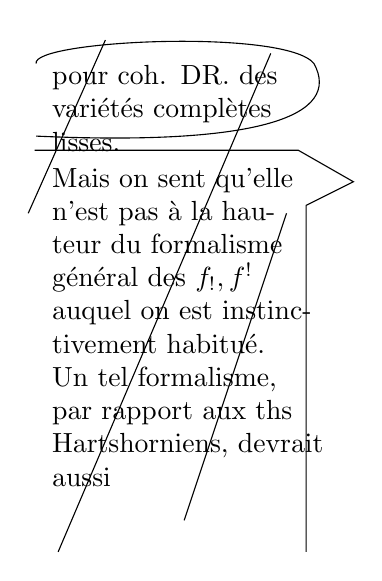
\begin{tikzpicture}[x=1cm,y=1cm]
\node[align=left,text width=3.4cm,anchor=north west] at (0,0) {\deleted{pour coh. DR. des variétés complètes \unsure{lisses}.}};
\draw (-.08,-.10) .. controls (-.15,.2) and (3.1,.35) .. (3.45,-.1) .. controls (3.8,-.75) and (2.8,-1.15) .. (-.08,-1.02);
\node[align=left,text width=3.5cm,anchor=north west] at (0,-1.3) {\deleted{Mais on sent qu'elle n'est pas à la hauteur du formalisme général des $\unsure{f_!,f^!}$ auquel on est \unsure{instinctivement} habitué. Un tel formalisme, \unsure{par rapport aux ths Hartshorniens}, devrait \unsure{aussi}}};
\draw (-.1,-1.2)--(3.25,-1.2)--(3.95,-1.6)--(3.35,-1.9)--(3.35,-6.3);
\draw (.8,.2)--(-.18,-2.0);
\draw (2.9,.03)--(.2,-6.3);
\draw (3.1,-2.0)--(1.8,-5.9);
\end{tikzpicture}}}

\deleted{\unsure{b)}} En car. $\unsure{0}$, pour \unsure{les variétés non singulières}, on trouve des invariants excellents, donnant en particulier les ``bons'' nombres de Betti.
Mais en car $p$, c'est moins raisonnable, car
1°) Si $X$ n'est pas propre, on trouve en général des vectoriels de dim infinie
\[
\unsure{\text{p. ex.}|\text{Ex.}}\qquad H_{\mathrm{DR}}^0(X)\simeq H^0(X,\underline O_X)^p\ ;
\]
2°) Même si $X$ est propre, on ne trouve pas en général les ``bons'' nombres de Betti ; par exemple on a
\[
\dim H_{\mathrm{DR}}^1(X)\ \deleted{\unsure{=}}\geq 2\dim\underline{\mathrm{Pic}}_X,
\]
et il y a des exemples où on a $>$, (dû vraisemblablement à des phénomènes de $p$-torsion $\ldots$).

Enfin 3°) Même dans des cas (tels celui des VA) où les $\dim H_{\mathrm{DR}}^i(X)\deleted{\unsure{=b^i(X)}}$ sont les ``bons'' $b^i(X)$, un défaut majeur de ces \unsure{esp. v.} (déjà signalé par Serre) c'est que le corps de
\margin{22}

\scanpage{24}
\mspage{4}
définition est de car $p>0$, et donc ils ne se prêtent pas à la détermination des nbs \uline{exacts} de p$^{\mathrm{ts}}$ fixes par formule de Lefschetz (mais seulement le nb mod $p$), donc \unsure{non plus} à une fondation satisfaisante des conjectures de Weil.

b) Le point de vue De Rham classique, \inserted{pour exprimer la coh. ``complexe'',} est trop exclusivement lié aux variétés \uline{non} singulières. Rien n'empêche évidemment de considérer aussi le complexe $\underline\Omega_X^\bullet$ et $\mathbb H^*(X,\Omega_X^\bullet)$ si $X$ est quelconque. Mais $\overline{\mathrm m}$ si $X$ est une courbe, affine ou complète, sur $\mathbb C$,
\deleted{singulière}
\inserted{p.ex. la droite affine ou projective \deleted{\unsure{qui a un point double}} un p$^{\mathrm t}$ de \unsure{rebr.} ordinaire,}
\deleted{(\unsure{disons unibranche si on y tient})}, on n'obtient déjà pas pour \deleted{\unsure{la}} $\dim H_{\mathrm{DR}}^1(X)$ le premier nb de Betti comme il faudrait.
On peut décider qu'on ne s'intéresse qu'aux variétés algébriques non singulières — mais l'expérience apprend que $\overline{\mathrm m}$ pour étudier celles-ci, on ne peut éviter l'introduction des variétés singulières, p.ex. à titre de fibres intervenant dans des \deleted{\unsure{fibrations}} morphismes
\margin{23}

\scanpage{25}
\mspage{5}
des schémas $\overline{\mathrm m}$ lisses. \deleted{\unsure{i.e.}}
\diagram{\begin{tikzcd}[ampersand replacement=\&]
f:X \arrow[r,dash] \& Y.
\end{tikzcd}}

Ainsi, connaissant déjà $H^*(X^{\mathrm{an}},\mathbb C)$ comme $H_{\mathrm{DR}}^*(X)$, on aimerait une \deleted{interprétation}\inserted{construction} purement algébrique de la suite spectrale de Leray de
\diagram{\begin{tikzcd}[ampersand replacement=\&]
f^{\mathrm{an}}:X^{\mathrm{an}} \arrow[r,dash] \& Y^{\mathrm{an}}
\end{tikzcd}} :
\diagram{\begin{tikzcd}[ampersand replacement=\&]
H^*(X^{\mathrm{an}},\mathbb C) \&
E_2^{pq}=H^p(Y^{\mathrm{an}},\mathbb R^q f_*^{\mathrm{an}}(\mathbb C_{X^{\mathrm{an}}}))
\arrow[l,Rightarrow]
\end{tikzcd}}.

En fait, $\overline{\mathrm m}$ si $f$ est lisse, donc à fibres non singulières, une telle description n'est pas du tout claire en termes de ce qui a été vu jusqu'à maintenant.
\deleted{[les $\mathbb R^q f_*(\underline\Omega_{X/\mathbb C}^\bullet)$}
\inserted{Nous reviendrons sur ce point tout à l'heure.}
Un formalisme
\deleted{sont des faisceaux discrets sur $Y$, \unsure{pas des|par des}}
\figure{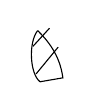
\begin{tikzpicture}[x=1cm,y=1cm]
\draw (0,0)..controls(-.12,-.15)and(-.1,-.55)..(.03,-.65);
\draw (.03,-.65)--(.32,-.6)..controls(.28,-.3)and(.12,-.12)..(0,0);
\draw (-.06,-.2)--(.15,.03);
\draw (-.02,-.55)--(.26,-.21);
\end{tikzpicture}}
\inserted{cohomologique} vraiment universel devrait impliquer, tt comme dans le cadre classique, l'écriture des suites spectrales de Leray — ce qui n'est possible que s'il englobe des ``faisceaux'' de coefficients de nature plus générale que les complexes de De Rham $\underline\Omega_X^\bullet$, — \inserted{englobant,} sans doute, également, des complexes d'opérateurs différentiels de nature plus générale que De Rham.

c) Du point de vue dualité et notions assimilées,
\margin{24}

\scanpage{26}
\mspage{6}
notons que pour des $X$ lisses et propres, on a bien le formalisme de dualité habituel (autodualité de $H_{\mathrm{DR}}(X)$, \inserted{d'où} \unsure{hom.} de Gysin, classe de coh. associée à un cycle alg, \deleted{\unsure{et}} compatibilité avec images directes, inverses, intersections) $\ldots$ le tout se faisant de façon tout analogue à ce que, dans le point de vue ``cohomologie de Hodge'' j'avais fait au Sém. Bourbaki.
Mais le ``lecteur informé'' au courant des histoires $f_!,f^!$ verra à quel point une \inserted{simple} dualité de ce type est \unsure{candide} et primaire.
On aimerait un formalisme $f_!,f^!$ du type de celui développé en long et en large dans le livre Hartshorne (Springer), \deleted{\unsure{et}} pour des morphismes $\pm$ quelconques, \inserted{disons \deleted{\unsure{propres,}}\inserted{séparés de} type fini;} de schémas.
Un tel formalisme, \inserted{impliquant des coeff. tels les complexes de D.R.,} devrait alors automatiquement donner \unsure{égal$^{\mathrm t}$} une description de l'\uline{homologie} singulière (comme il est suggéré par ailleurs dans mes papiers bleus$\ldots$).
Il y aurait lieu en particulier d'étendre ce formalisme, du cas de complexes à différentielles linéaires, au cas des complexes
\margin{25}

\scanpage{27}
\mspage{7}
à \inserted{différentielles des} op. différentiels.

Dans b) et c) reste posée, essentiellement, la question de la définition de la bonne \uline{catégorie de coefficients}, pour englober à la fois le formalisme des complexes \deleted{quasi} ``linéaires'' cohérents, et les complexes du type De Rham.
Les exposés que je fais doivent donner quelques indications plus précises sur la voie \deleted{\unsure{devons}}\deleted{\unsure{suivre}} dans laquelle il conviendra \deleted{de} probablement de chercher ces catégories de coefficients.

§ 2 \uline{Tour d'horizon sur les \deleted{autres} théories cohomologiques \inserted{$\ell$-adiques} pour les variétés algébriques}

\uline{a) Avantages}. \deleted{\unsure{Inconvénients}.}

On peut évidemment se demander : pourquoi à tout prix \deleted{désirer} aller jusqu'au bout dans un programme d'algébrisation \inserted{et de généralisation} à outrance de la cohomologie de De Rham.
On dispose déjà des invariants cohomologiques $\ell$-adiques, qui se prêtent à des applications \deleted{géométriques}
\margin{26}

\scanpage{28}
\mspage{8}
arithmétiques comme la formulation cohomologique des conjectures de Weil.
Faisons un petit tour d'horizon : à quoi on en est arrivé à ce sujet.

Si $X$ est une variété alg. sur un corps alg. clos $k$,
\deleted{propre sur $k$ pour fixer les idées.}
\inserted{\unsure{on|lui} associe pour tout $\ell$ nb premier}
\uline{$\ell\neq\operatorname{car} k$} des modules sur $\mathbb Z_\ell$
\[
H^i(X,\mathbb Z_\ell)=\varprojlim H^i(X_{\text{ét}},\mathbb Z/\ell^{\unsure{\nu}}\mathbb Z),
\]
dont le comportement pour $\ell$ \deleted{variable} fixé, $X$ variable, est à peu près celui de la cohomologie entière \inserted{ou} rationnelle dans le cadre transcendant.

Ainsi, si $k$ est le corps des complexes, le th. de comparaison nous fournit des isom can, fonctoriels en $X$
\[
\boxed{H^i(X,\mathbb Z_\ell)\simeq H^i(X^{\mathrm{an}},\mathbb Z)\otimes_{\mathbb Z}\mathbb Z_\ell}
\]
Ceci montre que \uline{la connaissance de la cohomologie entière transcendante de $X^{\mathrm{an}}$} (au moins du point de vue additif) \uline{est}
\margin{27}

\scanpage{29}
\mspage{9}
\deleted{\unsure{entièrement déterminée par}}
\inserted{\uline{équivalente à}}
\uline{la connaissance de}
\figure{\begin{tikzpicture}[baseline=(t.base)]
\node[draw,ellipse,inner sep=3pt] (t) {\uline{tous}};
\end{tikzpicture}}
\uline{les} $H^i(X,\mathbb Z_\ell)$.
De façon plus précise, pour un $\ell$ donné, la connaissance de $H^i(X,\mathbb Z_\ell)$ équivaut à celle du rang \inserted{$b_i(X)$} de $H^i(X^{\mathrm{an}},\mathbb Z)$, \inserted{c'est à dire de $H^i(X,\mathbb Z_\ell)$ sur $\mathbb Z_\ell$,} et de la composante $\ell$-primaire du sous-groupe de torsion de $H^i(X^{\mathrm{an}},\mathbb Z)$.

On obtient, en passant, par voie transcendante, le fait que si le corps de base $k$ est de car. $0$, alors les \inserted{$H^i(X,\mathbb Z_\ell)$ sont de t.f., leur rang,} $b_i(X,\mathbb Z_\ell)$ \deleted{est} pour $\ell$ variable est indépendant de $\ell$, et que pour $X$ fixé, seul$^{\mathrm t}$ pour un nb fini de $\ell$ \unsure{le} $\unsure{H^*|H^i}(X,\mathbb Z_\ell)$ a de la torsion.
Et par la $\overline{\mathrm m}$ voie, on trouve \inserted{p.ex.} que si on a un endom. $f$ de $X$, alors pour $i$ fixé, \deleted{l'ensemble} le polynôme caractéristique de l'endom. de $H^i(X,\mathbb Z_\ell)$
\margin{28}

\scanpage{30}
\mspage{10}
induit par $f$ est \uline{à coefficients entiers indépendants de $\ell$}

Situation beaucoup moins bonne en car. $p>0$, où on ne dispose pas de ``cohomologie entière'' transcendante.
Le fait que les $H^i(X,\mathbb Z_\ell)$ sont de t.f. (résultant de ce que les $H^i(X,\mathbb Z/\ell\mathbb Z)$ le sont) n'est prouvé que si $X$ est propre ou $\dim X\leq 2$ — pour l'avoir en général, il semble qu'il faille la résolution des singularités.
D'autre part, $\overline{\mathrm m}$ si $X$ est projectif et lisse, on ignore si p.ex. le rang de $H^2(X,\mathbb Z_\ell)$ est indépendant de $\ell$, et à fortiori, si le résultat plus haut pour les coefficients des polynômes caractéristiques est valable.
Cela semble actuellement, \inserted{d'ailleurs,} le \deleted{premier} plus important pas \unsure{restant} en direction d'une solution des conjectures de Weil.
\deleted{\unsure{Pour}} On peut commencer par tensoriser par $\mathbb Q_\ell$,
\margin{29}

\scanpage{31}
\mspage{11}

d'où des coefficients dans les $\mathbb Q_\ell$, et un premier problème est s'ils sont dans $\mathbb Q$. On sait (si $X$ est projectif non singulier) ramener ce pb à un pb de cycles algébriques du type Lefschetz.

Mais --- c'est là le ``\unsure{point}'' que je désire faire --- $\overline{\mathrm m}$ si ce pb ``\unsure{cru}'' \inserted{i.e. ``\unsure{non tordu}''} est résolu par l'affirmative, on \inserted{ne} pourra encore conclure que les coeff. sont des entiers, mais seulement \inserted{de $\mathbb Z[1/p]$, i.e.} de \deleted{entiers $\ell$-adiques} la forme $n/p^{\unsure{\delta}}$, avec $n\in\mathbb Z$. Ceci provient de la restriction
\[
\ell\ne\operatorname{car} k,
\]
de ce \uline{qu'il manque une théorie cohomologique $p$-adique pour les variétés algébriques en car. $p$}. Faute d'avoir une théorie de ce type, on ne saura

\margin{30}

\scanpage{32}
\mspage{12}

non plus comprendre les \uline{phénomènes de $p$-torsion cohomologique} des var. alg. en car. $p$. \unsure{D'autres} motivations \inserted{\unsure{pour voir vraiment complet}} ne manquent pas, \deleted{\unsure{peut-être}} \inserted{cf p.ex. l'exposé de Tate sur Brauer, \unsure{pour} heuristique d'une formule pour $\zeta$}

\margin{\uline{par exemple} des groupes de Brauer d'une \unsure{surface} sur un corps fini; \unsure{notre} \unsure{se heurte à} \unsure{un manque de connaissances} de \unsure{cohomologies} ``$p$-adiques'' \unsure{raisonnables}\ldots\ \unsure{ou le global}\ldots}

En analogie avec la coh. $\ell$-adique, on pourrait espérer trouver un foncteur
\diagram{\begin{tikzcd}[ampersand replacement=\&]
X \arrow[r,dash] \& H^i(X)
\end{tikzcd}}
de la catégorie des VA projectives lisses sur $k$, dans celle des modules de t.f. sur $\mathbb Z_p$, ou sur $\mathbb Q_p$, ayant les propriétés habituelles \deleted{\unsure{cf}} (Künneth, dualité, ``bons'' nbs de Betti \ldots). Un argument de Serre montre que déjà pour le $H^1$, et en se bornant aux $X$ \deleted{\unsure{de dim $\leq 2$}}, qui sont des VA de dim $\leq 2$, un tel foncteur n'existe pas. Il semble que l'anneau de coefficients naturel d'une coh. ``$p$-adique'' pour les var. sur un corps $k$ de car $p>0$, est plutôt l'anneau

\margin{31}

\scanpage{33}
\mspage{13}

$W(k)$ des vecteurs de Witt sur $k$, anneau de val. discrète dont le corps des fractions $W(k)[\frac1p]\supset\mathbb Q_p$ est un corps de car. \uline{nulle}.

Ceci devrait être le cas encore pour un corps de base \inserted{parfait} quelconque, non pas néc. alg. clos \ldots

\S 3 \uline{Revue des essais de définition d'une théorie \inserted{cohomologique} $p$-adique en car. $p>0$.}

\uline{Retour sur De Rham via Washnitzer Monsky.}

\inserted{\uline{Lien avec les stratifications de Gauss-Manin.}}

1) Utilisation des $p$-groupes éventuellement radiciels, \deleted{pour} comme coefficients pour la cohomologie (\unsure{pour|sur} la topologie plate).

Heuristiquement, cela marche magnifiquement en dim. 1, et \deleted{\illegible{3} \unsure{pour}} \inserted{on entrevoit une variante considérablement améliorée, de nature géométrique,} \deleted{\unsure{de la th}} en termes \unsure{du théorème|des théorèmes} de dualité en cohomologie plate, du corps de classes global géométrique (\unsure{constr.} sur un

\margin{32}

\scanpage{34}
\mspage{14}

corps, éventuellement fini). On espère que Raynaud tirera au clair cette théorie, et son analogue local --- ce qui exige d'ailleurs de surmonter des obstacles techniques considérables.

Mais en dim $n\geq 2$, c'est sans espoir, car Artin a remarqué que tous les \deleted{\unsure{$p$-groupes ét.}} groupes de coh. de $X$, à coeff. dans des $p$-groupes constants, s'annulent en dim $>n+1$. Donc \uline{en mettant les choses au mieux, on arrivera à construire des ``bons'' invariants cohomologiques par cette voie jusqu'en dim} $\dim X+1$ (et non $2\dim X$, qui est la bonne). Il faudra donc (si $X$ projective lisse) \inserted{\unsure{pour le moins}} compléter le tableau \unsure{par} heuristique par dualité de Poincaré \ldots\ On voit bien \uline{qu'il faudra}

\margin{33}

\scanpage{35}
\mspage{15}

\uline{une} \uuline{définition} \uline{de la coh. $p$-adique indépendante de la coh. plate}, \uline{quitte} \uuline{ensuite} \uline{à étudier ses relations (sans doute} fort intéressantes) \uline{avec cette dernière}.

2) \uline{L'approche de Washnitzer-Monsky.}

C'est dans cette approche qu'on voit la cohomologie de De Rham \deleted{qui} montrer à nouveau le bout de l'oreille ! Nous allons expliquer \inserted{pour le moment,} comment elle s'introduit dans l'approche de W-M., en \unsure{simplifiant} leur construction à l'extrême, (au risque de la défigurer \ldots !). On part de $X_0$ \unsure{projective} lisse sur $s$, \uline{on suppose} \inserted{\uline{d'abord}} qu'on puisse relever en $X$ \deleted{projective} propre et lisse sur $S=\operatorname{Spec}W(k)$, \deleted{soit $\eta$ le point générique}. Considérons le complexe $\underline{\Omega}_{X/S}^{\bullet}$, et

\margin{\diagram{\begin{tikzcd}[ampersand replacement=\&]
X_0 \arrow[r,phantom,"\subset"] \arrow[d,dash] \& X \arrow[d,dash]\\
s:\operatorname{Spec}k \arrow[r,phantom,"\subset"] \& S:\operatorname{Spec}W
\end{tikzcd}}}

\[
\boxed{H^i_{\mathrm{DR}}(X/S)=\mathbb H^i(X,\Omega^\bullet_{X/S})}
\]
C'est un module de t.f. sur $W(k)$.

\margin{34}

\scanpage{36}

\margin{\unsure{15|25}.11.66}

Nous avons montré que la cohomologie \deleted{de D.R.} \inserted{complexe ordinaire} d'une variété algébrique non singulière sur $\mathbb C$ \unsure{se décrit} par voie purement algébrique comme ``cohomologie de De Rham''
\[
H_{\mathrm{DR}}(X)=\mathbb H^*(X;\Omega_X^\bullet)
\]
\margin{\figure{\begin{tikzpicture}\draw (0,0)--(.24,.06);\end{tikzpicture}}}

Celle-ci a un sens pour n'importe quel schéma sur un corps quelconque. Cependant cette version de la cohomologie \unsure{nombreux} désavantages : liée aux formes diff donc aux variétés non sing, \inserted{le corps de \deleted{coefficient} base de la théorie coh. \unsure{peut} être de car $p>0$\ldots}

D'autre part, nous avons vu la désirabilité d'avoir une théorie de cohomologie ``$p$-adique'' pour les variétés en car. $p$, pour jouer le $\overline{\mathrm m}$ rôle que les \unsure{cohomologies} $\ell$-adiques, $\ell\ne p$. On veut les $\overline{\mathrm m}\mathrm s$ nbs de Betti etc \ldots

Une remarque sur la définition de la coh. de De Rham : $\underline{\Omega}^1_{X/S}$ est défini pour tt préschéma relatif $X/S$, et $\bigwedge^*\underline{\Omega}^1_{X/S}=\underline{\Omega}^*_{X/S}$ est muni d'un op. diff naturel\ldots\ On peut donc définir
\[
\left\{
\begin{aligned}
&H_{\mathrm{DR}}(X/S)=\mathbb H^*(X,\underline{\Omega}^*_{X/S})\\
&\text{et les }\mathbb R f_*(\underline{\Omega}^\bullet_{X/S})
\end{aligned}
\right.
\]

\margin{\figure{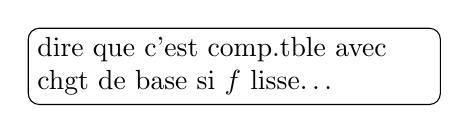
\begin{tikzpicture}
\node[draw,rounded corners,align=left,text width=5cm] at (0,0) {dire que c'est \unsure{comp.tble} avec chgt de base \unsure{si} $f$ \uline{lisse}\ldots};
\end{tikzpicture}}}

\margin{(coh. si $\left\{\begin{array}{l}
f\ \text{propre et }\unsure{\text{lisse}}\\
\text{ou }f\ \text{propre}, S\ \text{loc }\unsure{\text{noeth}}
\end{array}\right.$}

\margin{35}

\scanpage{37}

\uline{L'idée de} W-M. \deleted{serait} \inserted{\uline{semble pouvoir s'exprimer}} \uline{plus ou moins} \inserted{\uline{en disant}} \uline{que ce module est un invariant qui, à isom canonique près, ne dépend pas du choix du relèvement $X$ de $X_0$, et qui serait donc un invariant intrinsèquement attaché à $X_0$, qui serait alors par définition la cohomologie} \deleted{de D.R.} \uline{``$p$-adique'' \unsure{de celui-ci}.}

\margin{``\unsure{Some questions}'' \unsure{Journal Indien} 63/64\ldots}

\uline{Remarques} a) Cette construction marcherait aussi, mutatis mutandis, si on ne peut relever $X_0$ qu'en un \uline{schéma formel} lisse sur $S$.

b) D'après le texte publié de W-M, \deleted{il me semble qu'il} on pourrait \deleted{croire} être amené à penser que seul
\[
H^i_{\mathrm{DR}}(X/S)\otimes_W K
\]
\inserted{$K$ corps des fractions de $W$}
\deleted{\unsure{on}} devrait avoir la propriété d'invariance en question. De plus, la construction et la propriété invariance n'y sont traités que pour $X_0$ \uline{affine}

\margin{36}

\scanpage{38}

(et non propre), en utilisant un \unsure{relèvement} de $X_0$, non comme schéma ni comme schéma formel, mais en quelque chose qui ressemble à une \uline{variété rigide-analytique} à la Tate. De ce fait, il n'est défini, \inserted{dans $[\,]$} que des invariants \uline{locaux}. Par communication orale de W., il serait arrivé à définir des invariants globaux (sur $W$, et non seulement sur $K$), en travaillant \inserted{avec le complexe de De Rham} sur le \uline{site des relèvements de W.M} \deleted{(\illegible{3})} \uline{des ouverts affines}, et sauf erreur à justifier les assertions que \unsure{j'ai faites}.

c) On voit, grâce au th. de comparaison, que par cette construction (quand $X_0$ \unsure{se} relève en $X$ lisse sur $S$) on trouve des $H^i(X_0)$ qui donnent les bons nbs de Betti --- ce sont ceux de la fibre générique $X_t$ !

\margin{37}

\scanpage{39}

\uline{L'idée de W.M.}

\ldots\ldots

Donnons quelques détails sur ce que font \uline{réellement} W.M. Faute de pouvoir \unsure{relever} en général un $X_0$ lisse quelconque, on travaill. \inserted{\uline{d'abord}} avec des $X_0$ \uline{affines}. On sait (SGA 1960/61, $\overline{\underline{\mathrm{III}}}$) que un tel $X_0$ se relève de proche en proche en un $\mathfrak X$ \uline{formel} \inserted{\uline{lisse}} sur $\mathfrak S=\operatorname{Spf}W(k)$, \inserted{unique à isom (\uline{non unique}) près,} la première idée serait de prendre $\Omega^\bullet_{\mathfrak X/\mathfrak S}$ défini par passage à la limite à partir des $\Omega^\bullet_{X_n/W_n}$, et de poser
\[
H(X_{\unsure{0|m}})=\mathbb H^*(\mathfrak X,\Omega^\bullet_{\mathfrak X/\mathfrak S})
=H^*(\Gamma(\mathfrak X,\Omega^\bullet_{\mathfrak X/S})\unsure{)}
\]

Mais montrons que cela ne donne pas du tout ce qu'il faut, $\overline{\mathrm m}$ si $X_0=\operatorname{Spec} k[T]$ est la droite affine, donc
\[
\mathfrak X=\operatorname{Spf}
\underbrace{W\{t\}}_{\varprojlim W_n[T]}
\]
\inserted{séries formelles restreintes, i.e. à coeff. $\longrightarrow 0$.}
On voudrait trouver en effet que
\[
\mathbb H^1(\mathfrak X,\Omega^\bullet_{\mathfrak X/S})=0
\]

\margin{38}

\scanpage{40}

ou tout au moins que le premier mb. soit de torsion. En fait, il est de \uline{rang infini} sur $W$ !
\[
\begin{aligned}
\mathbb H^1(\mathfrak X,\Omega^\bullet_{\mathfrak X/S})
&=\Omega^1(\mathfrak X/S)/d(\mathcal O(\mathfrak X/S))\\
&\simeq W\{t\}/\underbrace{\operatorname{Im}(f\rightsquigarrow f')}_{\substack{\text{séries formelles}\\\text{restreintes }\uline{\text{dérivées}}}}
\end{aligned}
\]
Or pour que $\sum a_n t^n$ soit une dérivée en $\sum b_n t^n$, il f. et s. que
\[
\sum\frac1{n+1}a_n t^{n+1}
\]
\inserted{ou aussi $\sum\frac1n a_{n-1}t^n$}
soit encore une série formelle restreinte, i.e. que
\[
\unsure{v_p|\nu_p}(a_n)-\unsure{v_p|\nu_p}(n+1)\longrightarrow+\infty
\]
et comme $\unsure{v_p|\nu_p}(n)$ (quand $n$ variable) peut prendre des valeurs arbitrairement grandes, on voit qu'il ne suffit pas que
\[
\unsure{v_p|\nu_p}(a_n)\longrightarrow+\infty\quad !
\]

En notations multiplicatives, si $|\ |_{p}$ est la valeur absolue $p$-adique, \deleted{\unsure{on}} on veut que
\[
\frac{|a_n|_p}{|n+1|_p}\longrightarrow 0
\]
donc que
\[
|a_n|_p=\varepsilon_n|n+1|_p\qquad \varepsilon_n\longrightarrow 0
\]

\margin{39}

\scanpage{41}

C'est là une condition \inserted{de décroissance des coefficients} arithmétique assez biscornue. W.M. la remplacent par une condition plus forte, et plus maniable, savoir que
\[
|a_n|=O(1)\rho^n
\qquad
\begin{gathered}
\text{pour un }\rho>1\\
\text{convenable (dépendant de la suite }(a_n)\text{)}
\end{gathered}
\]
Cela signifie qu'au lieu de regarder l'anneau $W\{t\}$ des séries convergentes sur le disque unité \inserted{de $\overline K$ ($K$ corps des fractions de $W$)}, ils regardent l'anneau \inserted{$W^{\unsure{\dagger|+}}\{t\}$} des séries convergentes sur un disque de rayon $\rho>1$ \deleted{(\unsure{de rayon arbitraire}} un peu plus grand (dépendant de la fonction envisagée), On définit de même $W^{\unsure{\dagger|+}}\{t_1,\ldots,t_n\}$, et les \deleted{\unsure{anneaux}} W-M-algèbres, \deleted{de W.M} qui sont les quotients de tels anneaux par des idéaux \deleted{quelconques} fermés quelconques \deleted{(\unsure{fermés}} (les idéaux sont-ils

\margin{40}

\scanpage{42}

automatiquement fermés). \deleted{W.M. prouvent}

Il semble que le théorème suivant soit vrai (dont W.M. prouvent une variante un peu affaiblie) :

a) Si $A_0$ de t.f. sur $k$ est lisse sur $k$, $\exists A$ \inserted{W-M}-Algèbre sur $W$, \uline{plate} sur $W$, et un $k$-isomorphisme
\[
\varphi:A\otimes_W k\simeq A_0.
\]

b) De plus, un tel couple $(A,\varphi)$ est unique à isom (non unique près), i.e. si on a des \deleted{\unsure{cf}} $\overline{\mathrm m}$ $(A',\varphi')$, il existe un $W$-isom $u:A\longrightarrow A'$ rendant comm. le diagramme

\margin{\unsure{faire figure|faire preuve}.}

c) Définissons \inserted{pour tte Algèbre de W.M. $A$ sur $W$,} $\Omega^1(A/W)$ par la propriété universelle pour les dérivations de $A/W$ dans un $A$-module de type fini, d'où
\[
\Omega^*(A/W)=\bigwedge^*(A/W),
\]
qui est un \uline{complexe} de $W$-Algèbres.

\margin{\figure{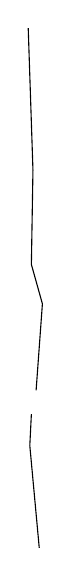
\begin{tikzpicture}
\draw (0,0)--(.06,-1.8)--(.04,-3)--(.18,-3.5)--(.10,-4.6);
\draw (.04,-4.9)--(.02,-5.3)--(.14,-6.6);
\end{tikzpicture}}}

\deleted{\unsure{pour deux} \unsure{soient} \inserted{$A,A'$} $(A,\varphi)$ $(A',\varphi')$ \inserted{et} comme en}

\deleted{b) et \unsure{choisissons} $u:A\overset{\sim}{\longrightarrow}A'$ comme en}

\deleted{\unsure{isom}}

b) $u:A\longrightarrow A'$ un hom de W.M-Algèbres lisses sur $W$, d'où
\diagram{\begin{tikzcd}[ampersand replacement=\&]
u^*:H^i(\Omega^\bullet(A'/W)) \arrow[r,dash] \& H^i(\Omega^*(A'/W))
\end{tikzcd}}

\margin{41}

\scanpage{43}

Cet homomorphisme ne dépend que de l'homomorphisme $u_0:A_0-A'_0$ induit sur les algèbres réduites mod $p$.
\margin{\figure{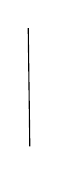
\begin{tikzpicture}\draw (0,0)--(.02,-1.5);\end{tikzpicture}}}

\uline{Cor} Si $A$ est un relèvement de W.M. \inserted{lisse} de $A_0$ lisse sur $k$, alors $H^i(\Omega^\bullet(A/W))$ ne dépend, à isom can. près, que de $A_0$.

En fait, W-M. ne prouvent ces résultats que pour des $A_0$ ``spéciales'', mais il y en a assez de celles-ci. De plus, dans leurs notes ils ne prouvent la propriété d'invariance c) que mod torsion, i.e. en tensorisant par $K$.

\deleted{\unsure{Si}} Lorsque $X_0$ est un schéma lisse quelconque sur $k$, utilisant ces résultats, W.M. définissent \inserted{dans $[\,]$} des ``faisceaux de coh.'' \deleted{$H^*(X$} $\mathcal H^*_{X_0}$ sur $X_0$, qui sont des faisceaux de $W$-modules.

Cela ne donne pas encore d'invariants

\margin{42}

\scanpage{44}

globaux, comme on en voudrait. \deleted{Dernièrement} \inserted{Récemment} W.M. ont utilisé la notion de \deleted{topos} site pour définir des invariants globaux : \uline{site des relèvements de} W.M. \uline{des ouverts affines spéciaux}, pour la ``topologie de Zariski''. Sur ce site les $\Omega^\bullet_{A/k}$ forment un complexe de faisceaux, dont ils prennent l'hypercohomologie. Ils trouvent des invariants globaux intrinsèques, qui sont des modules sur $W$. Ils vérifient (?) que dans le cas envisagé au début, ils retrouvent bien $\mathbb H^*(\mathfrak X,\underline{\Omega}^\bullet_{\mathfrak X/S})$, d'où la propriété d'invariance que j'y avais énoncée.

\figure{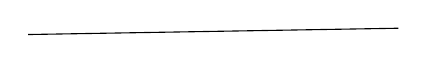
\begin{tikzpicture}\draw (0,0)--(4.7,.08);\end{tikzpicture}}

3) Critique de W.M.

C'est une idée nouvelle importante, en ce qu'elle met en relations la coh. de D.R. en car. 0, avec la cohomologie $p$-adique hypothétique, \unsure{p} Elle fournit une théorie cohomologique ``$p$-adique en car $p$'', qui échappe à une des critiques principales qu'on avait faite à D.R. naïve : elle

\margin{43}

\scanpage{45}

a comme anneau de coeff. $W(k)$, dont le corps des fractions $K$ est de car. 0, et non $k$. De plus, cette approche \deleted{ne} \inserted{(s'il est vrai qu'elle marche sur $W(k)$, pas seulement $K$)} \deleted{est} fournit \deleted{des relations satisfaisantes} une notion de torsion $p$-adique, \deleted{entre la cohomologie} qui est peut-être la bonne : est-ce la torsion $p$-adique de la fibre générique\deleted{?} géométrique ? Ici est \unsure{resoulevée} la question, extrêmement importante et profonde, des relations entre la cohomologie de D.R. et la cohomologie $p$-adique, quand on spécialise de la car. 0 à la car. $p>0$. (question déjà envisagée par Tate, \inserted{dans un langage différent,} dans son \unsure{séminaire} l'an dernier dans le \inserted{cas des} $H^1$ tout au moins).

Sur l'importance de cette question \deleted{\unsure{et}} pour l'attaque de certains pbs liés aux \inserted{familles de} cycles algébriques, cf mes papiers aux Inventiones \inserted{$[\,]$} à paraître prochainement.

\margin{44}

\scanpage{46}
Je \unsure{note|vois} cependant des \deleted{\unsure{graves}} critiques à formuler, la plus importante étant le rôle joué par les différentielles, ce qui pratiquement limite la théorie aux $X_0$ lisses.
Ne \deleted{\unsure{dispo}} travaillant qu'avec les seuls complexes $\Omega^\bullet_{X_t}$ de \deleted{différentielles} De Rham, \inserted{il est sans espoir que} cette approche \deleted{ne peut pas donner} \inserted{\unsure{fournisse|fournir}} des suites spectrales du \deleted{De Rham} type Leray pour un morphisme $f_0:X_0\to Y_0$, --- si précieuses pour faire des dévissages dans des démonstrations.

Comme conséquence de \deleted{\unsure{tout}} ceci, sans doute, W.M. n'ont pas été capables jusqu'à présent de prouver pour leur cohomologie les \deleted{\unsure{premières}} propriétés formelles les plus évidentes qu'on est en droit d'en attendre, notamment le fait que leurs $H^i_{\mathrm{WM}}(X)$ sont des modules de t.f. sur $W$ --- donc sans doute

\margin{45}

\scanpage{47}
non plus le théorème de dualité, ou de Künneth. \deleted{Je \unsure{ne} \unsure{d'autre part}}
(Il semble cependant que malgré cela, ils arrivent à utiliser leur cohomologie pour donner une expression à la Lefschetz-Weil de la fonction $\zeta$ d'un schéma projectif et lisse sur un corps fini, en montrant que les Frobenius opérant sur les $H^i(X)$ sont des opérateurs à trace .... ! Le formalisme semble alors proche de celui de Dwork, que je ne connais pas .... ).

\S\ \unsure{3} \inserted{\unsure{4)}} \uline{Relations \inserted{\uline{heuristique de} W.M.} avec mes idées de Gauss-Manin.}

1. Caractère assez surprenant à première vue de l'assertion d'invariance de W.M. \unsure{Supposons} p.ex. que l'on ait

\margin{46}

\scanpage{48}
une \unsure{pure|vraie} variation modulaire de $X_0$, s'exprimant disons par le fait que $X_0$ est la fibre, en un point $t_0$ au dessus du pt fermé $s$ de $S$, d'un schéma propre et lisse \inserted{$Y$} sur un $M$ de type fini sur $S$.
\margin{\figure{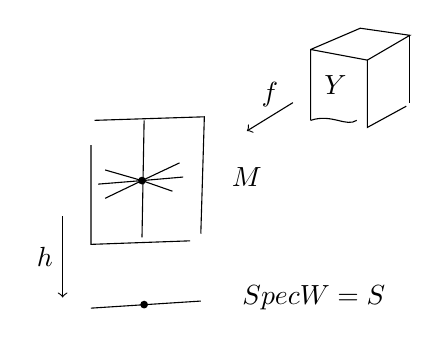
\begin{tikzpicture}[x=0.9cm,y=0.9cm]
\draw (3.5,3.3)--(3.5,4.3)--(4.2,4.6)--(4.9,4.5)--(4.3,4.15)--(3.5,4.3);
\draw (4.3,4.15)--(4.3,3.2)--(4.85,3.5);
\draw (4.9,4.5)--(4.9,3.55);
\draw (3.5,3.3)..controls(3.8,3.4)and(4.0,3.2)..(4.15,3.3);
\node at (3.85,3.8) {$Y$};
\draw[->] (3.25,3.55)--(2.6,3.15) node[midway,above] {$f$};
\draw (0.45,3.3)--(2.0,3.35)--(1.95,1.7);
\draw (0.4,2.95)--(0.4,1.55)--(1.8,1.6);
\draw (1.15,3.3)--(1.12,1.65);
\draw (0.6,2.6)--(1.12,2.45)--(1.65,2.7);
\draw (0.5,2.4)--(1.12,2.45)--(1.7,2.5);
\draw (0.6,2.2)--(1.12,2.45)--(1.55,2.3);
\fill (1.12,2.45) circle(1.4pt);
\node at (2.6,2.5) {$M$};
\draw[->] (0,1.95)--(0,0.8) node[midway,left] {$\unsure{h}$};
\draw (0.4,0.65)--(1.95,0.75);
\fill (1.15,0.7) circle(1.4pt);
\node[right] at (2.4,0.8) {$\operatorname{Spec}W=S$};
\end{tikzpicture}}}
Les différentes sections de $M$ sur $S$ donneront différentes façons de relever $X_0$ en un $X$ propre et lisse sur $S$. Prenant
\[
(*)\qquad K^\bullet=Rf_*(\underline{\Omega}^\bullet_{Y/M})
\]
on voit que pour \unsure{tte} telle section $g$ de $M$ sur $S$, définissant un $X_g^{\deleted{\unsure{g}}}$, et
\[
f_g^{\deleted{\unsure{g}}}:X_g^{\deleted{\unsure{g}}}\longrightarrow S
\]
\margin{$\unsure{\left(k+\frac12\right)\log(k+1)}
-\unsure{\left(k-\frac12\right)\log}$}
on a
\[
\mathbb{R}f_{g*}(\underline{\Omega}^*_{X_g/S})
\underset{\substack{\text{isom}\\\text{can}}}{\xleftarrow{\sim}}
g^*(K^\bullet)
\]
($g^*$ au sens des catégories dérivées ....). Il s'ensuit, \unsure{de même manière triviale}, que
\[
\mathbb{R}^if_{g*}(\underline{\Omega}^*_{X_g/S})
\xleftarrow{\sim}g^*(\mathcal{H}^i)
\]
\margin{47}

\scanpage{49}
\uline{Ainsi, on trouve que, \inserted{\uline{\unsure{posant|suivant}} \unsure{a)},} les complexes} $g^*(K^\bullet)$, \uline{pour les différentes sections} $g$ \uline{de} $M$ \uline{sur} $S$ \uline{passant par} $t_0$ \uline{sont can. isom. entre eux (au sens des cat. dérivées), donc les} $g^*(\mathcal{H}^i)$
(où $\mathcal{H}^i=\mathcal{H}^i(K^\bullet)$\inserted{$=\mathbb{R}^if_*(\underline{\Omega}^\bullet_{Y/M})$})
\uline{sont canoniquement isom. entre eux}, \deleted{\unsure{puis}} \uline{mod torsion}.
La donnée d'un tel système transitif d'isomorphismes peut être considérée comme une \uline{structure remarquable sur} $K^{\unsure{\bullet|*}}=\mathbb{R}f_*(\underline{\Omega}^\bullet_{Y/M})$ [\uline{en le point} $t_0$ relativement à la base $S$], ou sur les $\mathcal{H}^i=\mathbb{R}^if_*(\Omega^\bullet_{Y/M})$,
\deleted{Une telle}
\deleted{structure est \illegible{2} autrement}
d'espèce voisine à une \uline{structure de descente}.
Une structure de \deleted{\unsure{cet}} ce dernier type, \inserted{sur un Module $\underline{E}$ disons,} à supposer qu'elle soit effective, i.e. définisse un isom
\[
\underline{E}\ \deleted{\unsure{\mathcal{H}^i}}\simeq h^*(\underline{E}_0)
\]
($\underline{E}_0$ un Module sur $S$], définit une

\margin{48}

\scanpage{50}
tel système transitif d'isomorphismes entre les $g^*(\underline{E})$.
Nous allons décrire une structure, \inserted{un peu} moins forte que celle de descente, qui définit encore un tel système transitif d'isom: la \uline{structure de stratification sur $\underline{E}$, relativement à} $S$.

2. Définition générale d'une stratification.
\inserted{Relations avec connexions.}

3. Système transitif d'isom qu'elle fournit, si on est sur un anneau local complet.

4. La \deleted{\unsure{théorie de|idée de}} connexion de Gauss-Manin.

\margin{49}

\scanpage{51}
Dans le cas où $k$ est de car. 0, cela nous donne une connexion intégrable absolue sur $\underline{H}^*$ (Manin n'utilise pas ce langage géométrique).
Puis, dans le cas du $H^1$, et lorsque \deleted{$X$ est} provient d'un modèle \inserted{propre} lisse, Manin montre de façon assez compliquée que
$H^1(X,\Omega^\bullet_{X/k})$ (qui est $\subset H^1_{\mathrm{DR}}(X/k)$) est stable par les opérateurs $\Theta_X$.

3.5. En fait, par des arguments très simples directs, \deleted{qui} reposant sur la ``formule d'homotopie'' de Cartan
\[
d i_X+i_X d=\Theta_X
\]
on peut montrer, pour un morphisme $f:X\longrightarrow S$:

(i) Pour toute dérivation $\xi$ de $\underline{\Theta}_S$ qui se remonte, \deleted{\unsure{$X$}}, \inserted{loc. au dessus de $S$,} en une dérivation $\bar{\xi}$ de $\underline{\Theta}_X$ [condition tjrs satisfaite si $X$ est \deleted{\unsure{à}} \uline{formellement lisse sur $S$} et \uline{affine} sur $S$]
l'effet de $(\bar{\xi},\xi)$ opérant sur $\deleted{\unsure{\mathbb{R}}}f_*(\underline{\Omega}^\bullet_{X/S})$, est indépendant \uline{mod homotopie} \deleted{de} du choix de $\bar{\xi}$, donc dépend seulement de $\xi$; donc en particulier, \inserted{si $f$ form$^{\mathrm{t}}$ lisse et affine,} les
$\mathcal{H}^i(f_*(\Omega^\bullet_{X/S}))\unsure{=|\equiv}\mathbb{R}^if_*(\Omega^\bullet_{X/S})$
sont des Modules sur lesquels les dérivations de $S$ opèrent, --- et on vérifie les lois de linéarité et de crochet facilement.
Si $S$ lisse sur un $T$, ceci donne sur $\unsure{f_*|\mathbb{R}f_*}(\Omega^\bullet_{X/S})$ et sur les $\mathbb{R}^if_*(\Omega^\bullet_{X/S})$ des conn. intégrables rel/$T$.

\margin{50}

\scanpage{52}
(ii) Par une construction reposant \unsure{ess$^{\mathrm{t}}$.} sur les $\overline{\mathrm m}$ principes, mais sans doute un peu plus sophistiquée techniquement, (cf appendice), on trouve que si $f$ est lisse \unsure{qu. cpt} et qu. sép., alors
\[
\mathbb{R}f_*(\Omega^\bullet_{X/S})
\]
est muni d'une \uline{connexion absolue canonique} [au sens des catégories dérivées].
Cela ne signifie pas tt. à fait que les $\mathbb{R}^if_*(\Omega^\bullet_{X/S})$ sont munis individuellement de connexions absolues; c'est pourtant vrai si $S$ de car. 0, et $f$ propre et lisse (car alors la formation des $\mathbb{R}^i\unsure{f_*|f}(\Omega^\bullet_{X/S})$ eux-mêmes commute à l'extension de la base ....) --- ou encore, bien sûr, dans le cas lisse affine envisagé en (i)....
La vérification (pour $f$ propre, lisse) que cette connexion est compatible avec la construction transcendante, est en fait triviale.

\uline{Remarques}. On \unsure{pouvait|pourrait} espérer que ces connexions canoniques proviennent en fait de \uline{stratifications} canoniques, de façon que l'on aurait ainsi

\margin{51}

\scanpage{53}
explication ``à priori'' de l'\deleted{construction de} \inserted{invariance} affirmée par Washnitzer-Monsky.
C'est bien vrai si $S$ est de car. zéro, mais malheureusement c'est faux en car $p>0$, $\overline{\mathrm m}$ si on considère pour $f$ des projections structurales de \inserted{familles de} courbes elliptiques (= \unsure{schém.} elliptiques)!
\unsure{Il} s'agit donc pour le moment d'une relation heuristique et sentimentale, entre deux idées différentes, dont les relations exactes restent \deleted{\unsure{pour}} \inserted{loin} encore \inserted{d'avoir} été bien élucidées .....

\figure{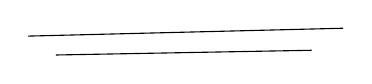
\begin{tikzpicture}
\draw (0,0)--(4.0,0.1);
\draw (0.35,-0.24)--(3.6,-0.18);
\end{tikzpicture}}

Pour résumer, on se trouve \unsure{actuellement} devant un puzzle, où il s'agit de reconstituer une théorie d'ensemble \deleted{\unsure{tenant compte}} \deleted{et} combinant

a) Une théorie cohomologique des complexes d'opérateurs différentiels, \deleted{qui} (notamment en vue d'application aux complexes de DR)

b) Une étude systématique des structures stratifiées, notamment \inserted{\unsure{mod. cohérents ou espaces fibrés}} \unsure{celles} qui \unsure{s'introduisent|à titre dérivé}

c) La théorie de Washnitzer-Monsky.

\margin{52}

\scanpage{54}
\S\ 4 \uline{Topos stratifiant et topos cristallin.}

4.1. Interprétation d'une stratification relative d'un Module $\underline{F}$ sur $X/S$.
Si \unsure{on a} une telle stratification, alors pour tt morphisme $f:\unsure{Y}\to X$, et tt voisinage infinitésimal $Y'$ de $Y$, \inserted{(sur $S$)} \deleted{\unsure{qui que}} tel que $f$ veut bien se prolonger (localement au moins) en $f':Y'\mathbin{-}X$, un système \uline{transitif} d'isom entre les $f'^*(\underline{F})$.
\margin{\diagram{\begin{tikzcd}[ampersand replacement=\&]
X \arrow[dd,dash] \& \unsure{Y_0|Y} \arrow[l,"f"'] \arrow[d,{Hooks[right]}-] \\
\& \unsure{Y'_0|Y'} \arrow[ul,"f'"]\\
S \&
\end{tikzcd}}}
On peut donc dire que la \deleted{\unsure{donnée}} \inserted{donnée d'une} stratification \deleted{\unsure{nous}} \inserted{revient à la} donnée \deleted{\unsure{canonique}}, pour tt voisinage infinitésimal $Y'$ d'un $Y\xrightarrow{f}X$, (sur $S$) \inserted{soumis à la condition déjà énoncée (autom. si $X/S$ form$^{\mathrm{t}}$ lisse)} d'un \uline{prolongement} \deleted{\unsure{can.}} de $F$ en un \uline{Module} sur $Y'$, avec des conditions de fonctorialité évidentes.
Pour exprimer plus commodément ce point de vue, et ses variantes, on va introduire des sites ad-hoc.

\margin{53}

\scanpage{55}
4.2. Définition des sites et des topos cristallins \inserted{de $X$ sur $S$}

Définition des sites et du topos stratifiant de $X$ sur $S$

C'est pareil si $X$ form$^{\mathrm{t}}$ lisse sur $S$.

\inserted{Ce sont des topos annelés}
\inserted{Attention, les sites \uline{n'ont pas en général d'objet final}!}
\deleted{Description d'un}
Ce sont des \deleted{\unsure{sites}} et topos \uline{annelés}.
Description des \deleted{un} faisceaux d'ensembles en termes de faisceaux habituels. Id. pour faisceaux d'anneaux, faisceaux de Modules sur faisceaux d'anneaux etc.

Faisceaux spéciaux: les hom de changement de base sont des isom.

\diagram{\[\begin{array}{l}
\text{Faisceaux de Modules spéciaux sur sites stratifiants}\\
\hfill\text{de }X/S\\
\rotatebox{90}{$\simeq$}\\
\text{Faisceaux de Modules à stratification sur }X/S.
\end{array}\]}

4.3. Énonçons de suite les résultats et conjectures suivants, qui seront \deleted{\unsure{établis}} détaillés plus tard:

\uline{Th} Si $S$ de car. 0 et $X$ lisse sur $S$, alors
\[
H^*_{\substack{\unsure{\mathrm{cris}/S}\\\text{ou strat}}}
(X/S,\underline{\mathcal{O}}_X)\simeq H^*_{\mathrm{DR}}(X/S)
\]
(isom can).
\deleted{\unsure{on a} $\unsure{f}=\mathbb{R}f_*(\mathcal{O}_X)$ \unsure{puis} $\uline{\unsure{H^i=0}}$, et
\[
(\mathbb{R}\unsure{f_{\mathrm{str}*}|f_*}(\mathcal{O}_X)^{\unsure{\mathrm{an}|\mathrm{ab}}}
\simeq\mathbb{R}f_*(\Omega^{\unsure{\bullet}}_{X/S})\quad ....]
\]}

\margin{54}

\scanpage{56}
\margin{Ceci donne une explication}

\uline{Conj.} Si $X$ loc. de t.f. sur $\mathbb{C}$, alors
\[
H^*_{\substack{\unsure{\mathrm{Str}}\\\text{ou crist.}}}
(X/\mathbb{C},\underline{\mathcal{O}}_X)
\simeq H^*(X^{\mathrm{an}},\mathbb{C})
\]

N.B. La conjecture est prouvée, grâce au th, \deleted{lorsque}, et au th. de comparaison de l'exposé 1, dans le cas où $X$ est lisse sur $\mathbb{C}$.
Donc \uline{dans le cas lisse, au dessus d'une base de} car. 0, \uline{on trouve une description de la coh. de} D.R. \uline{sans utiliser de différentielles}.

\margin{55}

\scanpage{57}
\margin{\figure{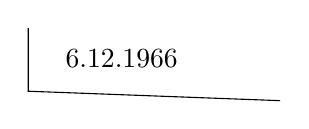
\begin{tikzpicture}
\draw (0,0.8)--(0,0)--(3.2,-0.12);
\node[anchor=west] at (0.35,0.42) {6.12.1966};
\end{tikzpicture}}}
\uline{Laïus}

\margin{\diagram{\begin{tikzcd}[ampersand replacement=\&]
X \arrow[d,"f"']\\
S
\end{tikzcd}}}
Soit $\mathcal{F}$ un Module quasi-cohérent stratifié sur $X/S$.
On a vu qu'il définit un module de $X_{\mathrm{strat}}$, et par là un faisceau cosimplicial
\inserted{\figure{\begin{tikzpicture}
\node[draw,ellipse,inner sep=4pt] {$\mathcal{F}^*=C(\mathcal{F})$};
\end{tikzpicture}}}
sur $X_{\mathrm{zar}}$, par
\[
C^n(\mathcal{F})=\mathcal{F}^{(n)}
=\varprojlim_i\mathcal{F}_{\Delta^n_{X/S}(i)}
\]
[pour n'importe laquelle des $n+1$ projections $\Delta^n_{X/S}(i)\to X$ on prend pour définir l'image inverse, il y a des isoms canoniques entre eux, précisément à cause de la stratification de $\mathcal{F}$].
On a
\[
\boxed{H^*(X_{\mathrm{str}},\mathcal{F})
\simeq\mathbb{H}^*(X_{\mathrm{zar}},C^*(\mathcal{F}))}
\]
On voit donc deux théories cohomologiques;
\deleted{\unsure{pour} \inserted{\unsure{chacune}} \unsure{aucune|encore} ne semble \illegible{1} à première vue, \unsure{purement} \illegible{3} \unsure{pour construire l'autre}.}

a) Pour un $\mathcal{F}$ quasi-cohérent sur $X$, on forme les $H^i(X_{\mathrm{zar}},\mathcal{F})$.

b) Si $\mathcal{F}$ est \uline{stratifié}, on forme les $H^i(X_{\mathrm{strat}},\mathcal{F})$, qui s'explicitent par la formule plus haut.

À première vue, le lien entre ces deux théories cohomologiques semble donné exclusivement par

\margin{56}

\scanpage{58}
la formule ci-dessus;
\deleted{\unsure{Il ne semble plus} \unsure{possible que}}
\inserted{À priori}, la cohomologie stratifiante d'un Module stratifié s'explicite comme une hypercohomologie zariskienne (et encore, dans un complexe dont la \deleted{\unsure{d}} différentielle n'est pas linéaire!), \deleted{et} mais l'inverse ne semble pas vrai.

On va voir pourtant que, dans un certain sens, il en est bien ainsi.
À peu de choses près, on associe à tt Module quasi-cohérent $\mathcal{F}$ (\uline{sans stratification}) un Module \deleted{quasi-cohérent} \inserted{(plutôt un pro-Module pro-quasi-cohérent)} $Q^0(\mathcal{F})$ stratifié, dont la cohomologie stratifiante est la coh. zariskienne \uline{ordinaire} de $X$.
De plus, $Q^0(\mathcal{F})$ est un foncteur en $\mathcal{F}$, non \unsure{seulement} pour des hom linéaires $\mathcal{F}\to\mathcal{G}$, mais $\overline{\mathrm m}$ \deleted{\unsure{pour} \illegible{1}} \inserted{(comme} faisceau \deleted{additif, $\overline{\mathrm m}$ de} d'$\mathcal{O}_X$-modules) pour des $\uline{D}:\mathcal{F}\unsure{\mathbin{-}|\to}\mathcal{G}$ qui sont seulement des op. diff. rel/$S$.
\margin{\figure{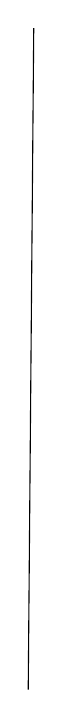
\begin{tikzpicture}
\draw (0,0)--(-0.07,-8.4);
\end{tikzpicture}}}
\deleted{\unsure{Il faut} \illegible{4}}
[Dans le cas très particulier où $\operatorname{diag}_{X/S}:X\longrightarrow X\times_S X$ est une immersion \unsure{nilpotente}, donc \deleted{\unsure{can.} $Q^0($} stratification /$S$ = donnée de descente à $S$, $Q^0(\mathcal{F})=f^*f_*(\mathcal{F})$].

L'intérêt \inserted{de ces divers points} est que \uline{l'hypercoh.} \inserted{zariskienne ordinaire} d'un complexe d'op. diff. \uline{peut s'interpréter comme la coh. stratifiante du complexe} correspondant de faisceaux stratifiés...!

\margin{57}

\scanpage{59}
les \uline{op. diff.} de $M$ dans $N$ (rel à $S$),

Alors, on trouve encore un foncteur en $M$, mais \deleted{tout} non à valeurs dans les $P^i$-Modules, mais \inserted{\figure{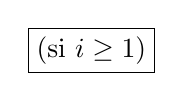
\begin{tikzpicture}
\node[draw,inner sep=3pt] {(si $i\geq1$)};
\end{tikzpicture}}}
seulement dans les $P^{i-1}$-Modules, où on considère $P^i[M]$ comme $P^{i-1}$-Module par \uline{restriction des scalaires} à l'aide de $\alpha^{i-1}:P^{i-1}\longrightarrow P^i$.
\inserted{(On le note alors $Q^{i-1}[M]$)}
En particulier, $Q^0[M]$ est \deleted{\unsure{le}} un foncteur en
$M\in\operatorname{Ob}\operatorname{Mod}(X/S)$
\inserted{[Modules sur $\mathcal{O}_X$, avec comme hom les op. diff. \deleted{d'ordre} rel. à $S$]},
à valeurs dans les pro-$\mathcal{O}_X$-Modules.
\margin{et qu'on utilise comme morphismes de \deleted{\unsure{type}} $\mathbb{N}$-pro-objets ceux de Artin--Riesz
[\unsure{ce qui revient à ne considérer} que des op. diff. de degré borné, --- qui est autom. si $X$ qu. cpt].}

\deleted{[$P^0[M]=M$ \deleted{\unsure{est}} \unsure{doit} être considéré comme un foncteur à valeurs dans $\operatorname{Ab}(X)$]}

Notons que l'hom $\unsure{\alpha^\bullet|\alpha^*}:P^*\mathbin{-}(SP)^*=Q^*$ permet de considérer $Q^*$ comme \deleted{\unsure{module}} \inserted{algèbre} \deleted{\unsure{pro}} cosimplicial sur l'\deleted{\unsure{anneau}} cosimplicial $P^*$, et que les opérations extrêmes droites

\margin{\figure{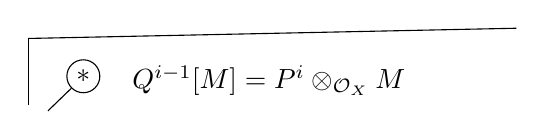
\begin{tikzpicture}
\draw (0,0.7)--(0,-0.15);
\draw (0,0.7)--(6.2,0.83);
\node[draw,circle,inner sep=1.8pt] (star) at (0.7,0.22) {$*$};
\draw (star.south west)--(0.25,-0.22);
\node[anchor=west] at (1.2,0.17) {$Q^{i-1}[M]=P^i\otimes_{\mathcal{O}_X}M$};
\end{tikzpicture}}}
\margin{58}

\scanpage{60}
\S 1 Ch. de De Rham ordinaire

\S 2 Tour d'horizon sur Ch. $\ell$-adiques. Motivations pour le désir d'une coh. $p$-adique en car. $p$.

\S 3 \unsure{Tapis} de Washnitzer-Monsky.

\S 4 Stratifications. Relations de W.M. avec connexions de Gauss-Manin sur coh. de De Rham

\S 5 \deleted{\unsure{Le}} Site cristallin et site stratifiant. Énoncé \deleted{de} d'un théorème et d'une conjecture en car. nulle.

\S 6 Calculs \v{C}echistes (car. quelconque).

\S 7 Comparaison de la Ch. de De Rham et cristalline (car. \unsure{nulle}).

\S 8 \deleted{Comparaison} \inserted{Retour} sur le cas de la car. $p>0$

\figure{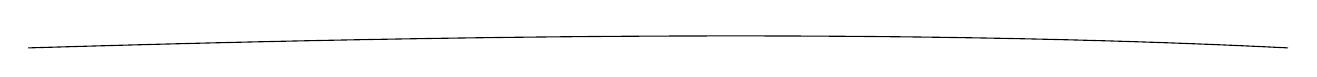
\begin{tikzpicture}
\draw (0,0) .. controls (5,.15) and (11,.25) .. (16,0);
\end{tikzpicture}}

\margin{\deleted{\uline{\unsure{Ch. strat.}}}\\
\uline{Ch. stratifiante}}

6.1. Commençons à travailler sur le topos \uline{stratifiant} pour $X/S$. Il y a l'objet $\widetilde X$ de ce topos: il \uline{couvre l'objet final} (c'est ici qu'on utilise la restriction sur les objets du site stratifiant par rapport à ceux du site cristallin). Donc suite spectrale de Leray
\[
H^*(X_{\mathrm{strat}},F)\Longleftarrow E_2^{pq}
=H^p(\nu\mapsto H^q(\widetilde X^{\nu+1},F)).
\]
Or on constate que
\figure{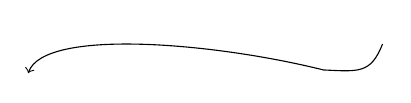
\begin{tikzpicture}
\draw[->] (4.5,.25)..controls (4.35,-.13) and (4.2,-.1)..(3.75,-.08)..controls (2.35,.27) and (.2,.45)..(0,-.12);
\end{tikzpicture}}
\[
\widetilde X^{\unsure{\nu}+1}
=\varinjlim_i\deleted{\unsure{\widetilde X}}\,
\underbrace{\Delta_X^{(\unsure{\nu})}(i)}_{
\substack{\text{voisinage inf. ième}\\
\text{de la diagonale dans}\\
X^{\nu+1}}}
\,\deleted{\unsure{X}}.
\]
\inserted{considéré comme \unsure{pro-objet} de $X$}
\deleted{$\unsure{X\longrightarrow}$}
\diagram{\begin{tikzcd}[ampersand replacement=\&,column sep=small,row sep=small]
X \& U\arrow[l]\arrow[dr] \&\\
\&\&X'
\end{tikzcd}}

D'autre part, pour tt objet $(U,X')$ du site stratifiant, on \unsure{aura}

\margin{59}
